\documentclass[11pt,a4paper]{report}
% --- Core ---
\usepackage[utf8]{inputenc}
\usepackage[T1]{fontenc}
\usepackage{lmodern}
\usepackage[margin=2.5cm]{geometry}
\usepackage{enumitem}

% --- Math & Symbols ---
\usepackage{amsmath, amssymb, amsfonts}

% --- UI & Layout ---
\usepackage{parskip} % Spasi antar paragraf, tanpa indentasi
\usepackage{float}
\usepackage{graphicx}
\usepackage{caption}
\usepackage{subcaption} % Untuk sub-figures
\usepackage{booktabs}   % Tabel cantik ( \toprule, \midrule, \bottomrule )
\usepackage{array}
\usepackage{tabularx}
\usepackage{multirow}
\usepackage{longtable}

% --- Colors & Links ---
\usepackage[dvipsnames]{xcolor}
\usepackage{hyperref}

% --- Code Snippets (Listings) ---
\usepackage{listings}
\definecolor{codegreen}{rgb}{0,0.6,0}
\definecolor{codegray}{rgb}{0.5,0.5,0.5}
\definecolor{codepurple}{rgb}{0.58,0,0.82}
\definecolor{backcolour}{rgb}{0.95,0.95,0.92}

\lstset{
    backgroundcolor=\color{backcolour},
    commentstyle=\color{codegreen},
    keywordstyle=\color{magenta},
    numberstyle=\tiny\color{codegray},
    stringstyle=\color{codepurple},
    basicstyle=\ttfamily\small,
    breakatwhitespace=false,
    breaklines=true,
    captionpos=b,
    keepspaces=true,
    numbers=left,
    numbersep=5pt,
    showspaces=false,
    showstringspaces=false,
    showtabs=false,
    tabsize=4
}

% --- Diagrams (TikZ) ---
\usepackage{tikz}
\usetikzlibrary{arrows.meta, shapes.geometric, shapes.misc, positioning, calc, fit, backgrounds, matrix, decorations.pathreplacing}

\tikzset{
    blok/.style={rectangle, draw, rounded corners=2pt, fill=blue!6, align=center, minimum height=0.8cm, font=\small},
    blokgol/.style={blok, fill=green!12},
    blokspn/.style={blok, fill=orange!14},
    blokkunci/.style={blok, fill=violet!10},
    data/.style={rectangle, draw, fill=gray!8, align=center, minimum height=0.7cm, font=\small},
    keputusan/.style={diamond, draw, aspect=2, fill=yellow!12, align=center, font=\small, inner sep=1pt},
    xorop/.style={circle, draw, inner sep=0pt, minimum size=0.45cm, path picture={
        \draw (path picture bounding box.north) -- (path picture bounding box.south)
              (path picture bounding box.west) -- (path picture bounding box.east);}},
    addop/.style={rectangle, draw, inner sep=0pt, minimum size=0.42cm, path picture={
        \draw (path picture bounding box.north) -- (path picture bounding box.south)
              (path picture bounding box.west) -- (path picture bounding box.east);}},
    panah/.style={-Stealth, thick},
    garis/.style={thick},
}

% --- Header & Footer ---
\usepackage{fancyhdr}
\pagestyle{fancy}
\fancyhf{}
\fancyhead[L]{\small IF4020 Kriptografi -- \algname}
\fancyhead[R]{\small \leftmark}
\fancyfoot[C]{\thepage}
\setlength{\headheight}{14pt}

% --- Referencing ---
\usepackage[noabbrev, capitalize]{cleveref}
\graphicspath{{images/}}

\renewcommand{\contentsname}{Daftar Isi}
\renewcommand{\listfigurename}{Daftar Gambar}
\renewcommand{\listtablename}{Daftar Tabel}
\renewcommand{\chaptername}{Bab}
\renewcommand{\appendixname}{Lampiran}
\renewcommand{\figurename}{Gambar}
\renewcommand{\tablename}{Tabel}
\renewcommand{\bibname}{Daftar Pustaka}
\renewcommand{\lstlistingname}{Kode}

\crefname{chapter}{Bab}{Bab}
\crefname{section}{Subbab}{Subbab}
\crefname{subsection}{Subbab}{Subbab}
\crefname{figure}{Gambar}{Gambar}
\crefname{table}{Tabel}{Tabel}
\crefname{equation}{Persamaan}{Persamaan}
\crefname{lstlisting}{Kode}{Kode}
\crefname{listing}{Kode}{Kode}
\crefname{appendix}{Lampiran}{Lampiran}
\crefname{enumi}{Langkah}{Langkah}

% --- Notasi ---
\newcommand{\algname}{Pregnant\_\allowbreak Sister}
\newcolumntype{Y}{>{\raggedright\arraybackslash}X}
\setlength{\emergencystretch}{3em}
\newcommand{\isi}[1]{\textcolor{red}{\textbf{[#1]}}}
\newcommand{\code}[1]{\texttt{#1}}
\newcommand{\rotl}{\mathbin{\lll}}

% build-remote.bat mengemas src/ di samping main.tex; kompilasi lokal membaca ../../src
\IfFileExists{src/feistel.py}{\def\srcdir{src}}{\def\srcdir{../../src}}


\hypersetup{
    colorlinks=true,
    linkcolor=black,
    citecolor=blue!60!black,
    filecolor=magenta,
    urlcolor=cyan!50!black,
    pdftitle={Laporan Tugas 2 IF4020 Kriptografi - Pregnant_Sister},
}

\newcommand{\anggotasatu}{M Rayhan Farrukh}
\newcommand{\nimsatu}{13523035}
\newcommand{\anggotadua}{Darrel Adinarya S}
\newcommand{\nimdua}{13523061}
\newcommand{\anggotatiga}{Rhio Bimo Prakoso S}
\newcommand{\nimtiga}{13523123}
\newcommand{\anggotaempat}{Frederiko Eldad M}
\newcommand{\nimempat}{13523147}

\begin{document}

\begin{titlepage}
    \centering

    \Large \textsf{Laporan Tugas 2 IF4020 Kriptografi} \\[0.3cm]
    \large \textsf{Perancangan Block Cipher Baru} \\
    \vspace{1.2cm}

    {\Huge \textbf{\algname}} \\[0.4cm]
    \large \textit{Block Cipher 256-bit Berbasis Cellular Automaton\\(Conway's Game of Life) dan Jaringan Feistel Hibrida} \\
    \vspace{1.2cm}

    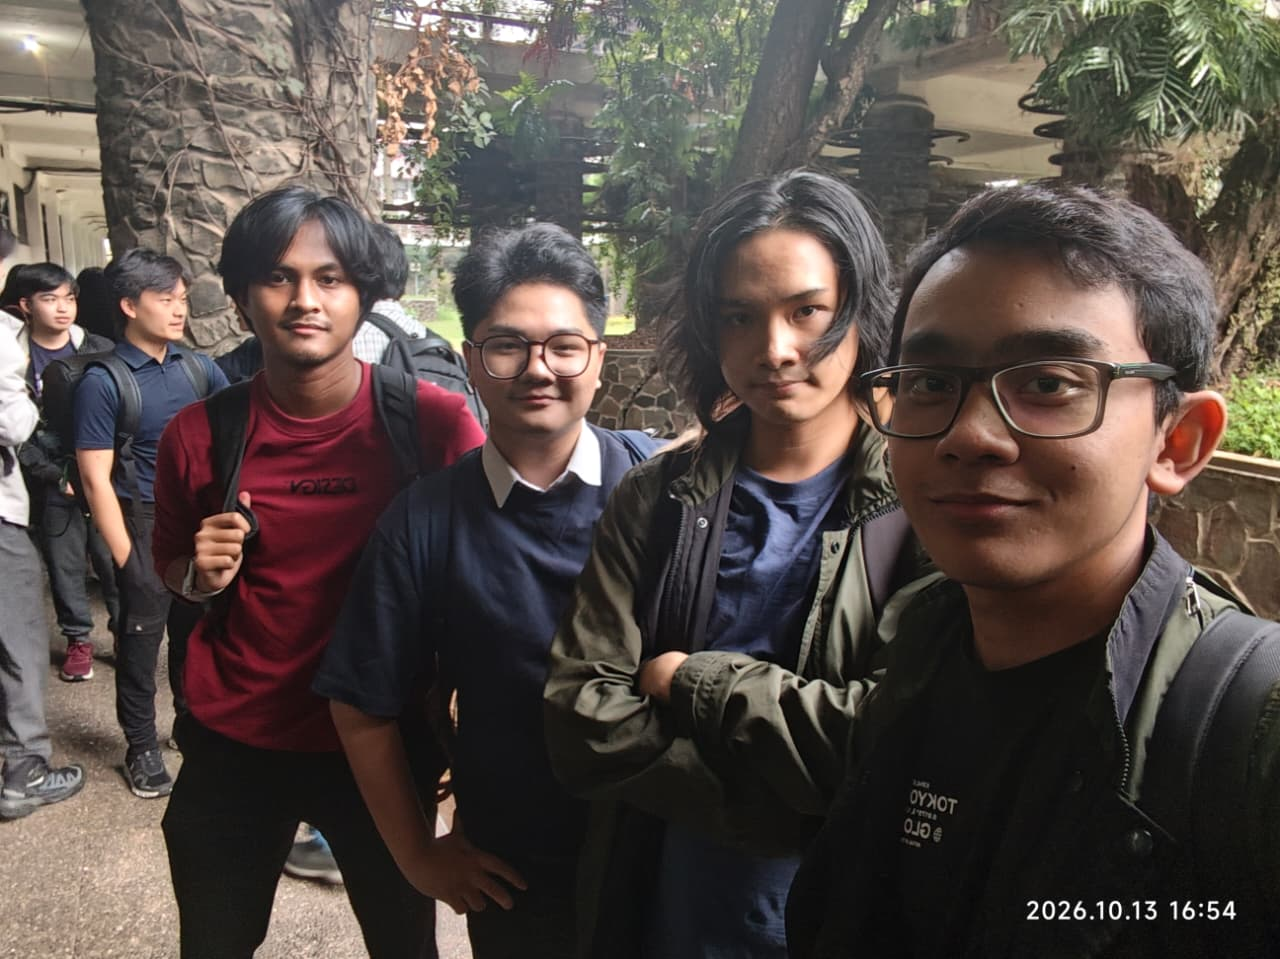
\includegraphics[width=0.62\textwidth, height=6.8cm, keepaspectratio]{cover.jpeg} \\
    \vspace{1.0cm}

    \large \textit{Disusun oleh:} \\[0.3cm]
    \begin{tabular}{l l}
        \anggotasatu  & \nimsatu \\
        \anggotadua   & \nimdua \\
        \anggotatiga  & \nimtiga \\
        \anggotaempat & \nimempat
    \end{tabular}

    \vfill

    \large
    Program Studi Teknik Informatika \\
    Sekolah Teknik Elektro dan Informatika \\
    Institut Teknologi Bandung \\
    2026
\end{titlepage}

\ifnum0\pdffilesize{images/pernyataan.pdf}>0
    \AddToHookNext{shipout/background}{\put(0,-\paperheight){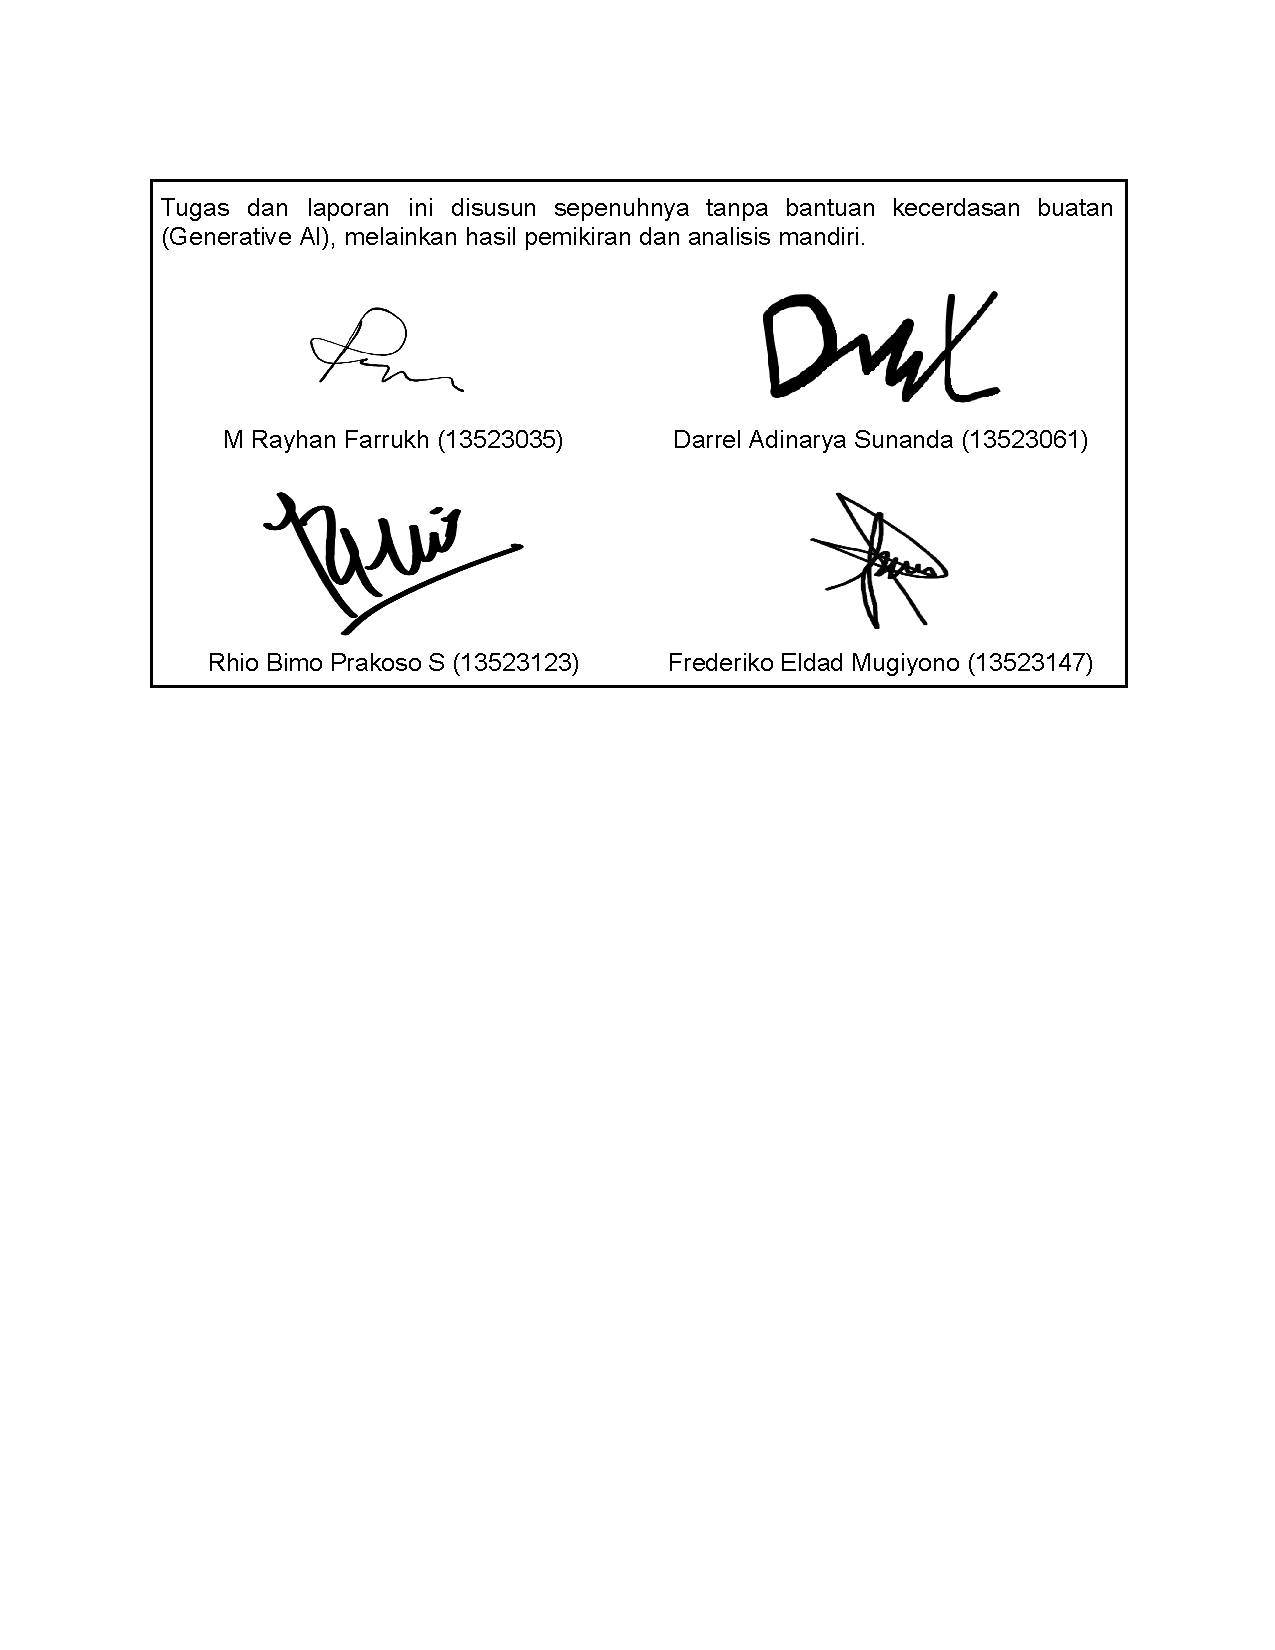
\includegraphics[width=\paperwidth,height=\paperheight]{pernyataan.pdf}}}%
    \thispagestyle{empty}\null
\else
    \thispagestyle{empty}
    \vspace*{\fill}
    \begin{center}
        \isi{Halaman pernyataan}\\[0.2cm]
        \small ganti \code{docs/tex/images/pernyataan.pdf} MANA HALAMAN PERNYATAANYA WOIIII
    \end{center}
    \vspace*{\fill}
\fi
\clearpage

\pagenumbering{roman}
\tableofcontents
\listoffigures
\listoftables
\newpage

\pagenumbering{arabic}
\setcounter{page}{1}

\chapter{Pendahuluan}

\section{Latar Belakang}
\textit{Block cipher} adalah primitif kriptografi kunci simetris yang mengenkripsi data dalam satuan blok berukuran tetap. Hampir semua protokol pengamanan data modern, mulai dari TLS, enkripsi diska, hingga pesan instan, bergantung pada \textit{block cipher} yang dipadukan dengan mode operasi tertentu. Keamanan sebuah \textit{block cipher} ditentukan oleh seberapa baik ia mewujudkan dua prinsip Shannon \cite{shannon1949}, yaitu \textit{confusion} (hubungan antara kunci dan \textit{ciphertext} dibuat serumit mungkin) dan \textit{diffusion} (pengaruh satu bit \textit{plaintext} disebar ke sebanyak mungkin bit \textit{ciphertext}).

Rancangan \textit{block cipher} yang dipakai saat ini umumnya menggunakan komponen yang sudah dipelajari secara mendalam, seperti Kotak-S, permutasi, dan operasi aritmetika modular. Di sisi lain, \textit{cellular automaton} (CA) telah lama diusulkan sebagai sumber ketidakteraturan untuk kriptografi \cite{wolfram1986}. CA terdiri atas sel-sel sederhana yang diperbarui berdasarkan aturan lokal, tetapi dapat menghasilkan perilaku global yang kompleks dan sulit diprediksi. Conway's Game of Life (GoL) \cite{gardner1970} adalah CA dua dimensi yang paling dikenal. Aturannya sangat sederhana (B3/S23), tetapi perilakunya cukup kompleks sehingga GoL terbukti \textit{Turing-complete}.

Tugas ini meminta perancangan sebuah \textit{block cipher} baru beserta implementasi, simulasi pada berbagai mode operasi, dan analisis keamanannya. Kelompok kami merancang \textbf{\algname}, yaitu \textit{block cipher} 256-bit yang memadukan GoL dengan komponen \textit{block cipher} klasik di dalam jaringan Feistel. Laporan ini menjelaskan rancangan tersebut, hasil pengujiannya, serta kelebihan dan kelemahan yang kami temukan.

\section{Tinjauan Singkat Block Cipher Pembanding}

\subsection{Data Encryption Standard (DES)}
DES distandardisasi oleh NIST pada tahun 1977 \cite{fips46}. DES memproses blok 64 bit dengan kunci efektif 56 bit melalui 16 ronde jaringan Feistel. Fungsi ronde DES terdiri atas ekspansi 32 bit menjadi 48 bit, XOR dengan \textit{round key}, delapan Kotak-S berukuran $6 \times 4$ bit, dan permutasi P. Struktur Feistel membuat proses dekripsi cukup dilakukan dengan menjalankan algoritma yang sama dengan urutan \textit{round key} terbalik. Kelemahan utama DES adalah ruang kuncinya yang kecil ($2^{56}$), sehingga kunci DES sudah dapat ditemukan dengan pencarian menyeluruh menggunakan perangkat keras khusus pada akhir 1990-an. DES juga rentan secara teoretis terhadap kriptanalisis diferensial \cite{biham1991} dan linear \cite{matsui1994}.

\subsection{Advanced Encryption Standard (AES)}
AES (Rijndael) \cite{fips197, daemen2002} menggantikan DES sejak 2001. AES memproses blok 128 bit dengan kunci 128, 192, atau 256 bit dalam 10, 12, atau 14 ronde. Berbeda dengan DES, AES menggunakan struktur \textit{Substitution--Permutation Network} (SPN). Setiap ronde terdiri atas \code{SubBytes} (Kotak-S $8 \times 8$ bit berbasis invers di GF($2^8$)), \code{ShiftRows}, \code{MixColumns} (perkalian matriks MDS di GF($2^8$)), dan \code{AddRoundKey}. Desain AES berlandaskan \textit{wide trail strategy} yang menjamin batas bawah jumlah Kotak-S aktif, sehingga peluang karakteristik diferensial dan linear dapat dibuktikan cukup kecil.

\subsection{RC6}
RC6 \cite{rivest1998} adalah finalis kompetisi AES yang memproses blok 128 bit dalam 20 ronde. Ciri khas RC6 (dan pendahulunya, RC5) adalah \textit{data-dependent rotation}: besar rotasi bit ditentukan oleh nilai data itu sendiri. RC6 juga memadukan operasi dari struktur aljabar yang berbeda, yaitu XOR, penjumlahan modulo $2^w$, dan perkalian bilangan bulat, sehingga sulit dianalisis dengan satu kerangka aljabar saja.

\subsection{Perbandingan}
\Cref{tab:perbandingan} merangkum perbandingan ketiga \textit{block cipher} di atas dengan rancangan \algname.

\begin{table}[H]
    \centering
    \caption{Perbandingan \algname{} dengan \textit{block cipher} sejenis}
    \label{tab:perbandingan}
    \small
    \begin{tabularx}{\textwidth}{l Y Y Y Y}
        \toprule
        \textbf{Aspek} & \textbf{DES} & \textbf{AES} & \textbf{RC6} & \textbf{\algname} \\
        \midrule
        Ukuran blok & 64 bit & 128 bit & 128 bit & 256 bit \\
        Panjang kunci & 56 bit & 128/192/256 bit & 128/192/256 bit & $\geq$ 256 bit (di-\textit{hash} SHA-256 menjadi 256 bit) \\
        Struktur & Feistel & SPN & Feistel tergeneralisasi & Feistel dengan dua jenis fungsi ronde \\
        Jumlah ronde & 16 & 10/12/14 & 20 & 18 (2 GoL + 16 SPN) \\
        Komponen nonlinear & 8 Kotak-S $6\times4$ & Kotak-S $8\times8$ & Rotasi bergantung data, perkalian & GoL, Kotak-S $8\times8$, penjumlahan mod 256, rotasi bergantung data \\
        Penjadwalan kunci & Permutasi dan rotasi & Ekspansi dengan Kotak-S & Ekspansi dengan konstanta & SHA-256 dan evolusi GoL dengan injeksi ulang \textit{nonce} dan \textit{whitening} \\
        \textit{Round key} per pesan & Tetap & Tetap & Tetap & Berbeda (bergantung \textit{nonce}) \\
        \bottomrule
    \end{tabularx}
\end{table}

\section{Gagasan Utama Rancangan}
Rancangan \algname{} berangkat dari pertanyaan: \textit{bagaimana memanfaatkan sifat kompleks Game of Life tanpa bergantung sepenuhnya pada GoL sebagai satu-satunya sumber keamanan?} Evolusi GoL tidak dapat dibalik (banyak konfigurasi berbeda dapat berevolusi ke konfigurasi yang sama). Sifat ini mustahil diterapkan pada SPN murni, tetapi justru tidak menjadi masalah di dalam jaringan Feistel, karena fungsi ronde Feistel tidak perlu memiliki invers. Berdasarkan pengamatan tersebut, kami menyusun lima gagasan utama.

\begin{enumerate}
    \item \textbf{Jaringan Feistel hibrida.} Blok 256 bit dibagi menjadi dua paruh 128 bit dan diproses dalam 18 ronde Feistel. Ronde pertama dan terakhir memakai fungsi ronde berbasis GoL ($f_{\text{GoL}}$), sedangkan ronde 2 sampai 17 memakai fungsi ronde SPN bergaya AES ($f_{\text{SPN}}$).
    \item \textbf{GoL di dalam fungsi ronde.} $f_{\text{GoL}}$ menyusun paruh blok sebagai grid $8 \times 16$ bit, lalu mengevolusikannya beberapa generasi pada grid toroidal. Untuk mengurangi tabrakan akibat sifat GoL yang tidak injektif, hasil evolusi di-XOR kembali dengan masukan.
    \item \textbf{Inti SPN yang teruji.} $f_{\text{SPN}}$ memakai Kotak-S, \code{ShiftRows}, dan \code{MixColumns} AES yang sifat diferensial dan linearnya sudah terbukti baik, lalu ditambah penjumlahan modulo 256 dengan kunci dan rotasi 128 bit yang besarnya bergantung pada data (terinspirasi RC6).
    \item \textbf{Penjadwalan kunci berbasis GoL.} Kunci di-\textit{hash} dengan SHA-256, dicampur dengan \textit{nonce}, diisikan secara spiral ke grid $16 \times 16$, lalu dievolusikan dengan GoL. Pada setiap ronde, pola baru dari kunci dan \textit{nonce} yang digeser diinjeksikan ulang ke grid sebelum evolusi, dan pola yang sama dipakai kembali untuk \textit{whitening} hasil evolusi sebelum dilipat menjadi \textit{round key}. Dengan demikian, 18 \textit{round key} saling berbeda dan bit-bitnya seimbang.
    \item \textbf{Round key unik per pesan.} \textit{Nonce} acak 32 byte dibangkitkan setiap kali enkripsi dan ikut menentukan \textit{round key}. Akibatnya, \textit{plaintext} dan kunci yang sama menghasilkan \textit{ciphertext} yang berbeda pada setiap enkripsi, bahkan pada mode ECB.
\end{enumerate}

\section{Tujuan}
Tujuan pengerjaan tugas ini adalah:
\begin{enumerate}
    \item merancang \textit{block cipher} baru yang memenuhi prinsip \textit{confusion} dan \textit{diffusion};
    \item mengimplementasikan algoritma tersebut beserta lima mode operasi (ECB, CBC, CFB, OFB, CTR) dan mekanisme \textit{padding};
    \item menguji kebenaran enkripsi dan dekripsi pada berkas teks dan biner; serta
    \item menganalisis keamanan rancangan melalui uji \textit{avalanche effect}, entropi, histogram, dan pengujian tambahan.
\end{enumerate}

\section{Sistematika Laporan}
\Cref{ch:dasar-teori} membahas dasar teori yang mendasari rancangan. \Cref{ch:perancangan} menjelaskan rancangan \algname{} secara rinci. \Cref{ch:implementasi} memaparkan implementasi dan hasil simulasi pada seluruh mode operasi. \Cref{ch:analisis} menganalisis keamanan rancangan. \Cref{ch:kesimpulan} berisi kesimpulan dan saran pengembangan.

\chapter{Dasar Teori}
\label{ch:dasar-teori}

\section{Block Cipher, Confusion, dan Diffusion}
\textit{Block cipher} adalah pasangan fungsi $E_K : \{0,1\}^n \to \{0,1\}^n$ dan $D_K = E_K^{-1}$ yang memetakan blok \textit{plaintext} berukuran $n$ bit ke blok \textit{ciphertext} berukuran sama di bawah kunci $K$ \cite{munir2026}. Shannon \cite{shannon1949} merumuskan dua prinsip perancangan:
\begin{itemize}
    \item \textbf{\textit{Confusion}}: hubungan statistik antara kunci dan \textit{ciphertext} dibuat serumit mungkin, umumnya dengan substitusi nonlinear (Kotak-S).
    \item \textbf{\textit{Diffusion}}: pengaruh setiap bit \textit{plaintext} dan kunci disebar ke banyak bit \textit{ciphertext}, umumnya dengan permutasi dan transformasi linear.
\end{itemize}
Keduanya diwujudkan dengan mengulang fungsi ronde sederhana sebanyak beberapa kali (\textit{product cipher}).

\section{Jaringan Feistel}
Jaringan Feistel \cite{feistel1973} membagi blok menjadi paruh kiri $L$ dan kanan $R$. Pada ronde ke-$i$ dengan \textit{round key} $K_i$:
\begin{equation}
    L_i = R_{i-1}, \qquad R_i = L_{i-1} \oplus F(R_{i-1}, K_i).
    \label{eq:feistel}
\end{equation}
Dekripsi menggunakan struktur yang sama dengan urutan \textit{round key} terbalik, karena $L_{i-1} = R_i \oplus F(L_i, K_i)$. Sifat terpenting struktur ini adalah \textbf{fungsi $F$ tidak perlu memiliki invers}. Fungsi apa pun, termasuk yang tidak injektif, tetap menghasilkan permutasi yang dapat dibalik. DES adalah contoh klasik \textit{cipher} Feistel \cite{fips46}.

\section{Substitution--Permutation Network dan Komponen AES}
SPN menerapkan substitusi dan permutasi secara langsung pada seluruh \textit{state}, sehingga setiap lapisan harus dapat dibalik. AES \cite{fips197, daemen2002} memakai empat transformasi pada \textit{state} $4 \times 4$ byte:
\begin{itemize}
    \item \code{SubBytes}: setiap byte $x$ diganti dengan $S(x) = A \cdot x^{-1} \oplus \texttt{0x63}$, dengan $x^{-1}$ invers perkalian di GF($2^8$) modulo $m(x) = x^8 + x^4 + x^3 + x + 1$ dan $A$ matriks afin. Kotak-S ini memiliki keseragaman diferensial 4 (peluang diferensial maksimum $2^{-6}$) dan bias linear maksimum $2^{-4}$.
    \item \code{ShiftRows}: baris ke-$i$ dirotasi ke kiri sejauh $i$ byte.
    \item \code{MixColumns}: setiap kolom dikalikan dengan matriks MDS $\left[\begin{smallmatrix}2&3&1&1\\1&2&3&1\\1&1&2&3\\3&1&1&2\end{smallmatrix}\right]$ di GF($2^8$), dengan \textit{branch number} 5.
    \item \code{AddRoundKey}: XOR \textit{state} dengan \textit{round key}.
\end{itemize}

\section{Cellular Automaton dan Conway's Game of Life}
\textit{Cellular automaton} (CA) adalah sistem dinamis diskret berupa kisi sel yang masing-masing memiliki keadaan berhingga. Semua sel diperbarui serentak menurut aturan lokal yang bergantung pada sel itu sendiri dan tetangganya. Game of Life (GoL) \cite{gardner1970} adalah CA dua dimensi biner dengan ketetanggaan Moore (8 tetangga) dan aturan B3/S23:
\begin{equation}
    s_{t+1} =
    \begin{cases}
        1 & \text{jika } N_t = 3, \text{ atau } s_t = 1 \text{ dan } N_t = 2,\\
        0 & \text{selainnya},
    \end{cases}
    \label{eq:gol}
\end{equation}
dengan $s_t$ keadaan sel dan $N_t$ jumlah tetangga yang hidup pada generasi $t$. Pada grid berhingga, batas toroidal (sisi kiri bersambung dengan sisi kanan, sisi atas dengan sisi bawah) membuat setiap sel memiliki tepat delapan tetangga. GoL bersifat \textbf{tidak dapat dibalik}: banyak konfigurasi tidak memiliki pendahulu (\textit{Garden of Eden}) dan banyak konfigurasi berbeda berevolusi ke keadaan yang sama.

\section{Related Works: Cellular Automaton dalam Kriptografi}
Wolfram \cite{wolfram1986} mengusulkan CA satu dimensi aturan 30 sebagai pembangkit bilangan acak semu untuk \textit{stream cipher}, dengan alasan bahwa evolusinya tampak acak walaupun aturannya sederhana. Nandi dkk.\ \cite{nandi1994} kemudian mengusulkan \textit{block cipher} dan \textit{stream cipher} berbasis CA yang dapat diprogram. Secara umum, penelitian kriptografi berbasis CA memanfaatkan dua sifat: paralelisme (semua sel dapat dihitung serentak) dan perilaku kompleks yang muncul dari aturan sederhana. Kelemahan yang sering dilaporkan adalah struktur linear pada aturan tertentu dan kecenderungan konfigurasi menuju keadaan stabil. Kedua kelemahan ini menjadi pertimbangan dalam rancangan kami. GoL dipilih karena aturannya nonlinear, dan GoL tidak dijadikan satu-satunya sumber nonlinearitas.

\section{Mode Operasi dan Padding}
Mode operasi menentukan cara \textit{block cipher} dipakai untuk pesan yang lebih panjang dari satu blok \cite{sp80038a}. Pada ECB, setiap blok dienkripsi secara independen. CBC meng-XOR setiap blok \textit{plaintext} dengan blok \textit{ciphertext} sebelumnya. CFB, OFB, dan CTR mengubah \textit{block cipher} menjadi \textit{stream cipher} dengan cara mengenkripsi umpan balik atau \textit{counter}, lalu meng-XOR hasilnya dengan \textit{plaintext}. Mode ECB dan CBC membutuhkan \textit{padding} agar panjang pesan menjadi kelipatan ukuran blok. Skema PKCS\#7 \cite{rfc5652} menambahkan $p$ byte bernilai $p$, dengan $1 \le p \le b$ untuk ukuran blok $b$ byte.

\section{Metrik Pengujian Keamanan}
\begin{itemize}
    \item \textbf{\textit{Avalanche effect}}: perubahan satu bit masukan (\textit{plaintext} atau kunci) idealnya mengubah sekitar 50\% bit keluaran. Kriteria yang lebih ketat, \textit{Strict Avalanche Criterion} (SAC) \cite{webster1986}, mensyaratkan setiap bit keluaran berubah dengan peluang tepat $\frac12$.
    \item \textbf{Entropi Shannon} \cite{shannon1948}: $H = -\sum_{i=0}^{255} p_i \log_2 p_i$ bit per byte, dengan $p_i$ frekuensi relatif nilai byte $i$. Nilai maksimum 8 dicapai saat seluruh nilai byte muncul dengan peluang sama.
    \item \textbf{Histogram dan uji $\chi^2$}: histogram \textit{ciphertext} yang baik tampak rata. Kerataannya dapat diuji dengan $\chi^2 = \sum_i (O_i - E_i)^2 / E_i$ dengan $E_i = N/256$. Pada 255 derajat kebebasan dan taraf nyata 5\%, nilai kritisnya adalah 293,25.
    \item \textbf{Keseragaman diferensial dan linear} Kotak-S \cite{biham1991, matsui1994, heys2002}: nilai maksimum pada \textit{Difference Distribution Table} (DDT) dan \textit{Linear Approximation Table} (LAT). Semakin kecil nilainya, semakin tahan Kotak-S terhadap kriptanalisis diferensial dan linear.
\end{itemize}

\chapter{Perancangan Block Cipher}
\label{ch:perancangan}

\section{Spesifikasi Umum}
\algname{} adalah \textit{block cipher} kunci simetris dengan spesifikasi seperti pada \cref{tab:spesifikasi}. Notasi yang dipakai di seluruh bab ini dirangkum pada \cref{tab:notasi}.

\begin{table}[H]
    \centering
    \caption{Spesifikasi \algname}
    \label{tab:spesifikasi}
    \begin{tabularx}{0.9\textwidth}{l Y}
        \toprule
        \textbf{Parameter} & \textbf{Nilai} \\
        \midrule
        Ukuran blok & 256 bit (32 byte), dibagi menjadi dua paruh 128 bit \\
        Panjang kunci & minimal 256 bit (32 byte); kunci di-\textit{hash} dengan SHA-256 menjadi 256 bit \\
        \textit{Nonce} & 256 bit (32 byte) acak dari CSPRNG, dibangkitkan setiap enkripsi \\
        Struktur & Jaringan Feistel 18 ronde \\
        Fungsi ronde & $f_{\text{GoL}}$ pada ronde 1 dan 18, $f_{\text{SPN}}$ pada ronde 2--17 \\
        \textit{Round key} & 18 buah, masing-masing 128 bit \\
        Penjadwalan kunci & SHA-256, lalu Game of Life $16 \times 16$ toroidal, 4 generasi per ronde, dengan injeksi ulang \textit{nonce} dan \textit{whitening} \\
        Mode operasi & ECB, CBC (bawaan), CFB, OFB, CTR \\
        \textit{Padding} & PKCS\#7 dengan ukuran blok 32 byte \\
        Keluaran & Base64$(\text{\textit{nonce}} \,\Vert\, C)$ \\
        \bottomrule
    \end{tabularx}
\end{table}

\begin{table}[H]
    \centering
    \caption{Notasi}
    \label{tab:notasi}
    \begin{tabularx}{0.9\textwidth}{l Y}
        \toprule
        \textbf{Notasi} & \textbf{Arti} \\
        \midrule
        $\oplus$ & XOR bit demi bit \\
        $\boxplus$ & penjumlahan per byte modulo 256 \\
        $x \rotl n$ & rotasi kiri $x$ sejauh $n$ bit \\
        $a \,\Vert\, b$ & penyambungan (konkatenasi) $a$ dan $b$ \\
        $L_i, R_i$ & paruh kiri dan kanan (masing-masing 128 bit) setelah ronde ke-$i$ \\
        $K_i$ & \textit{round key} ke-$i$ (128 bit), $1 \le i \le 18$ \\
        $N$ & \textit{nonce} 32 byte \\
        $\mathrm{GoL}^g(G)$ & hasil evolusi grid $G$ sebanyak $g$ generasi Game of Life \\
        \bottomrule
    \end{tabularx}
\end{table}

\section{Alur Global Enkripsi dan Dekripsi}
\Cref{fig:alur-global} memperlihatkan alur lengkap enkripsi sebuah pesan. Langkah-langkahnya adalah sebagai berikut.
\begin{enumerate}
    \item Kunci divalidasi (minimal 32 byte) dan data dikonversi menjadi \textit{bytes}.
    \item Data diberi \textit{padding} PKCS\#7 hingga panjangnya kelipatan 32 byte (\cref{sec:padding}).
    \item \textit{Nonce} 32 byte dibangkitkan secara acak.
    \item Penjadwalan kunci menurunkan 18 \textit{round key} dari kunci dan \textit{nonce} (\cref{sec:keysched}).
    \item Data dipotong menjadi blok 32 byte, lalu dienkripsi sesuai mode operasi (\cref{sec:mode}). Setiap pemanggilan $E$ menjalankan 18 ronde Feistel (\cref{sec:feistel}).
    \item \textit{Nonce} disambungkan di depan \textit{ciphertext}, lalu hasilnya dikodekan dengan Base64.
\end{enumerate}
Dekripsi menjalankan langkah sebaliknya: Base64 didekode, 32 byte pertama dibaca sebagai \textit{nonce}, \textit{round key} diturunkan ulang, setiap blok didekripsi sesuai mode, lalu \textit{padding} dibuang dan divalidasi.

\begin{figure}[H]
    \centering
    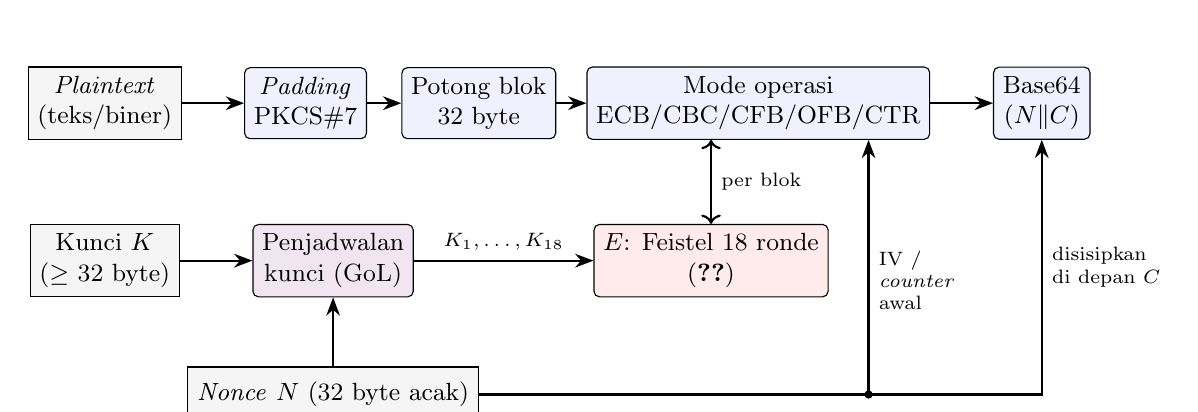
\begin{tikzpicture}[font=\small]
        \node[data] (pt) at (0,0) {\textit{Plaintext}\\(teks/biner)};
        \node[blok] (pad) at (2.55,0) {\textit{Padding}\\PKCS\#7};
        \node[blok] (split) at (4.75,0) {Potong blok\\32 byte};
        \node[blok, minimum width=3.6cm] (mode) at (8.3,0) {Mode operasi\\ECB/CBC/CFB/OFB/CTR};
        \node[blok] (b64) at (11.9,0) {Base64\\$(N \Vert C)$};

        \node[data] (key) at (0,-2) {Kunci $K$\\($\geq$ 32 byte)};
        \node[blokkunci] (ks) at (2.9,-2) {Penjadwalan\\kunci (GoL)};
        \node[blok, fill=red!8] (feistel) at (7.7,-2) {$E$: Feistel 18 ronde\\(\cref{fig:feistel})};
        \node[data] (nonce) at (2.9,-3.7) {\textit{Nonce} $N$ (32 byte acak)};

        \draw[panah] (pt) -- (pad);
        \draw[panah] (pad) -- (split);
        \draw[panah] (split) -- (mode);
        \draw[panah] (mode) -- (b64);
        \draw[panah] (key) -- (ks);
        \draw[panah] (nonce) -- (ks);
        \draw[panah] (ks) -- node[above, font=\scriptsize] {$K_1, \dots, K_{18}$} (feistel);
        \draw[panah, <->] (feistel.north) -- node[right, font=\scriptsize] {per blok} (feistel.north |- mode.south);
        \draw[panah] (nonce.east) -- (11.9,-3.7) -- node[pos=0.5, right, font=\scriptsize, align=left] {disisipkan\\di depan $C$} (b64.south);
        \fill (9.7,-3.7) circle (1.5pt);
        \draw[panah] (9.7,-3.7) -- node[pos=0.45, right, font=\scriptsize, align=left] {IV /\\\textit{counter}\\awal} ($(mode.south)+(1.4,0)$);
    \end{tikzpicture}
    \caption{Alur global enkripsi \algname}
    \label{fig:alur-global}
\end{figure}

\section{Jaringan Feistel 18 Ronde}
\label{sec:feistel}
Fungsi enkripsi satu blok $E$ memecah blok 256 bit $P$ menjadi $L_0 \Vert R_0$ (masing-masing 128 bit), lalu menjalankan 18 ronde Feistel:
\begin{equation}
    L_i = R_{i-1}, \qquad R_i = L_{i-1} \oplus F_i(R_{i-1}, K_i), \qquad
    F_i =
    \begin{cases}
        f_{\text{GoL}} & i \in \{1, 18\},\\
        f_{\text{SPN}} & 2 \le i \le 17.
    \end{cases}
    \label{eq:feistel-ps}
\end{equation}
Keluaran blok adalah $C = R_{18} \Vert L_{18}$, yaitu dengan pertukaran paruh terakhir dibatalkan seperti pada DES. Struktur ini diperlihatkan pada \cref{fig:feistel}.

Pemilihan fungsi ronde mengikuti peran masing-masing:
\begin{itemize}
    \item \textbf{Ronde 1 dan 18 ($f_{\text{GoL}}$)} berfungsi sebagai lapisan masuk dan keluar yang nonlinear dan berbeda sifat aljabarnya dari inti SPN. Penyerang yang ingin menganalisis inti SPN harus terlebih dahulu melewati transformasi GoL yang tidak memiliki deskripsi aljabar sederhana.
    \item \textbf{Ronde 2--17 ($f_{\text{SPN}}$)} memberikan jaminan \textit{confusion} dan \textit{diffusion} yang terukur melalui Kotak-S dan \code{MixColumns} AES.
\end{itemize}

\begin{figure}[H]
    \centering
    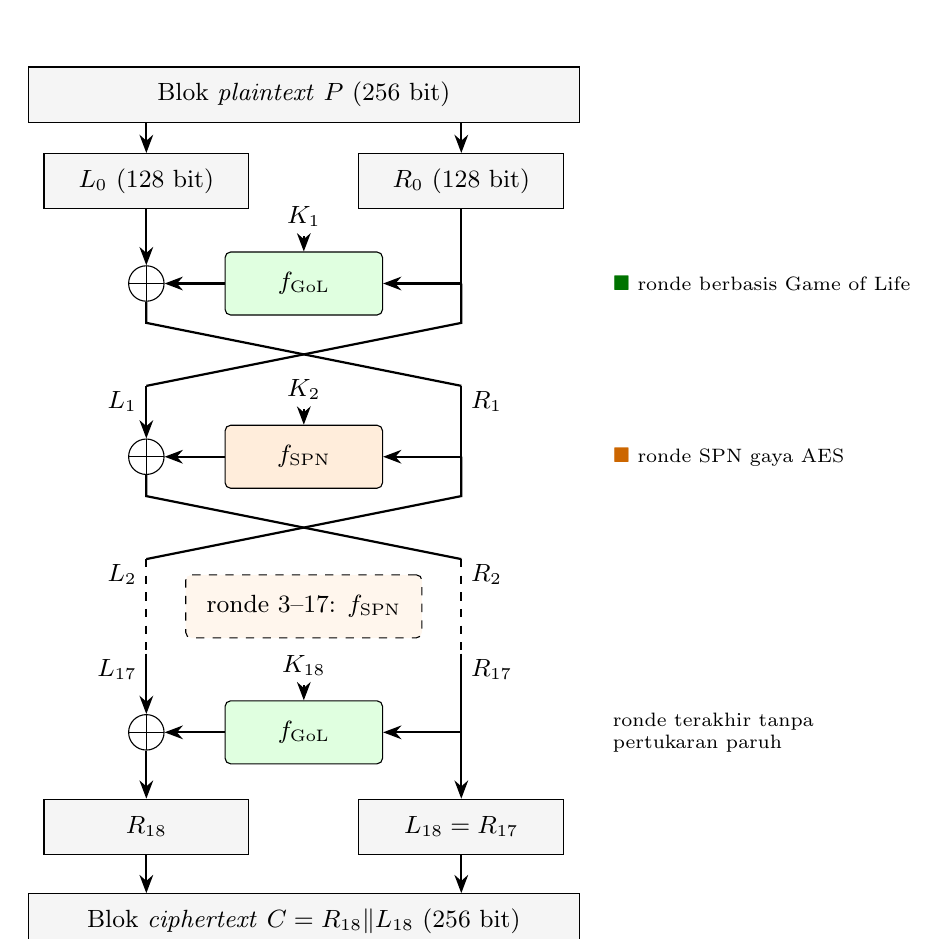
\begin{tikzpicture}[x=1cm, y=1cm, font=\small]
        \node[data, minimum width=7cm] (P) at (0,0) {Blok \textit{plaintext} $P$ (256 bit)};
        \node[data, minimum width=2.6cm] (L0) at (-2,-1.1) {$L_0$ (128 bit)};
        \node[data, minimum width=2.6cm] (R0) at (2,-1.1) {$R_0$ (128 bit)};
        \draw[panah] (P.south -| L0) -- (L0);
        \draw[panah] (P.south -| R0) -- (R0);

        % ronde 1
        \node[xorop] (x1) at (-2,-2.4) {};
        \node[blokgol, minimum width=2cm] (f1) at (0,-2.4) {$f_{\text{GoL}}$};
        \node (k1) at (0,-1.55) {$K_1$};
        \draw[panah] (L0) -- (x1);
        \draw[garis] (R0) -- (2,-2.4);
        \draw[panah] (2,-2.4) -- (f1);
        \draw[panah] (f1) -- (x1);
        \draw[panah] (k1) -- (f1);
        \draw[garis] (x1) -- (-2,-2.9) -- (2,-3.7);
        \draw[garis] (2,-2.4) -- (2,-2.9) -- (-2,-3.7);
        \node[left] at (-2,-3.9) {$L_1$};
        \node[right] at (2,-3.9) {$R_1$};

        % ronde 2
        \node[xorop] (x2) at (-2,-4.6) {};
        \node[blokspn, minimum width=2cm] (f2) at (0,-4.6) {$f_{\text{SPN}}$};
        \node (k2) at (0,-3.75) {$K_2$};
        \draw[panah] (-2,-3.7) -- (x2);
        \draw[garis] (2,-3.7) -- (2,-4.6);
        \draw[panah] (2,-4.6) -- (f2);
        \draw[panah] (f2) -- (x2);
        \draw[panah] (k2) -- (f2);
        \draw[garis] (x2) -- (-2,-5.1) -- (2,-5.9);
        \draw[garis] (2,-4.6) -- (2,-5.1) -- (-2,-5.9);
        \node[left] at (-2,-6.1) {$L_2$};
        \node[right] at (2,-6.1) {$R_2$};

        % ronde 3-17
        \draw[garis, dashed] (-2,-5.9) -- (-2,-7.1);
        \draw[garis, dashed] (2,-5.9) -- (2,-7.1);
        \node[blokspn, minimum width=3cm, fill=orange!7, dashed] at (0,-6.5) {ronde 3--17: $f_{\text{SPN}}$};
        \node[left] at (-2,-7.3) {$L_{17}$};
        \node[right] at (2,-7.3) {$R_{17}$};

        % ronde 18
        \node[xorop] (x18) at (-2,-8.1) {};
        \node[blokgol, minimum width=2cm] (f18) at (0,-8.1) {$f_{\text{GoL}}$};
        \node (k18) at (0,-7.25) {$K_{18}$};
        \draw[panah] (-2,-7.1) -- (x18);
        \draw[garis] (2,-7.1) -- (2,-8.1);
        \draw[panah] (2,-8.1) -- (f18);
        \draw[panah] (f18) -- (x18);
        \draw[panah] (k18) -- (f18);

        \node[data, minimum width=2.6cm] (R18) at (-2,-9.3) {$R_{18}$};
        \node[data, minimum width=2.6cm] (L18) at (2,-9.3) {$L_{18} = R_{17}$};
        \draw[panah] (x18) -- (R18);
        \draw[panah] (2,-8.1) -- (L18);
        \node[data, minimum width=7cm] (C) at (0,-10.5) {Blok \textit{ciphertext} $C = R_{18} \Vert L_{18}$ (256 bit)};
        \draw[panah] (R18) -- (R18 |- C.north);
        \draw[panah] (L18) -- (L18 |- C.north);

        \node[right, align=left, font=\scriptsize] at (3.8,-2.4) {\textcolor{green!45!black}{$\blacksquare$} ronde berbasis Game of Life};
        \node[right, align=left, font=\scriptsize] at (3.8,-4.6) {\textcolor{orange!80!black}{$\blacksquare$} ronde SPN gaya AES};
        \node[right, align=left, font=\scriptsize] at (3.8,-8.1) {ronde terakhir tanpa\\pertukaran paruh};
    \end{tikzpicture}
    \caption{Struktur jaringan Feistel 18 ronde pada \algname}
    \label{fig:feistel}
\end{figure}

\section{Fungsi Ronde \texorpdfstring{$f_{\text{GoL}}$}{f-GoL}}
\label{sec:fgol}
Fungsi ronde berbasis Game of Life didefinisikan sebagai
\begin{equation}
    f_{\text{GoL}}(R, K) = \mathrm{Ratakan}\big(\mathrm{GoL}^4(\mathrm{Grid}_{8\times16}(R \oplus K))\big) \oplus R.
    \label{eq:fgol}
\end{equation}
Langkah-langkahnya (\cref{fig:fgol}) adalah:
\begin{enumerate}
    \item \textbf{Pencampuran kunci.} $X = R \oplus K$ (128 bit).
    \item \textbf{Penyusunan grid.} 128 bit $X$ disusun menjadi grid 8 baris $\times$ 16 kolom secara \textit{big-endian}: dua byte pertama menjadi baris teratas, dan bit paling signifikan menjadi kolom paling kiri.
    \item \textbf{Evolusi.} Grid dievolusikan 4 generasi dengan aturan B3/S23 (\cref{eq:gol}) pada batas toroidal.
    \item \textbf{Perataan dan XOR umpan maju.} Grid hasil evolusi diratakan kembali menjadi 128 bit, lalu di-XOR dengan $R$.
\end{enumerate}

XOR umpan maju pada langkah terakhir penting karena evolusi GoL tidak injektif. Contoh ekstremnya, semua grid yang selnya mati atau terisolasi berevolusi menjadi grid kosong. Tanpa XOR dengan $R$, banyak nilai $R$ berbeda akan menghasilkan keluaran $F$ yang sama. Dengan XOR tersebut, dua masukan $R \neq R'$ yang tabrakan pada GoL tetap menghasilkan keluaran yang berbeda, karena selisihnya $R \oplus R'$ muncul langsung di keluaran.

\begin{figure}[H]
    \centering
    \begin{subfigure}[t]{0.47\textwidth}
        \centering
        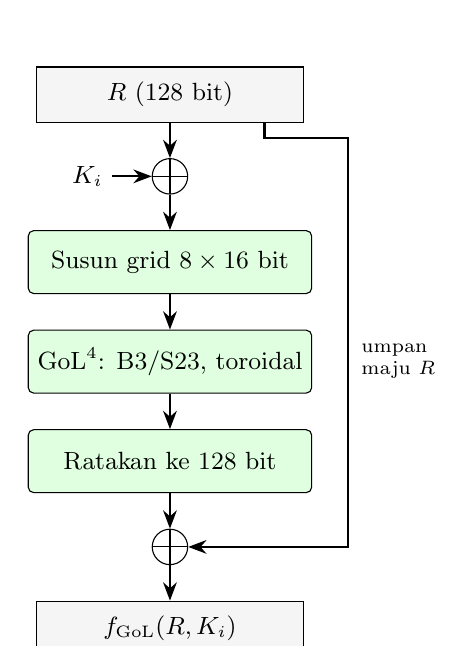
\begin{tikzpicture}[node distance=0.45cm, font=\small]
            \node[data, minimum width=3.4cm] (in) {$R$ (128 bit)};
            \node[xorop, below=of in] (x) {};
            \node[left=0.5cm of x] (k) {$K_i$};
            \node[blokgol, below=of x, minimum width=3.6cm] (grid) {Susun grid $8 \times 16$ bit};
            \node[blokgol, below=of grid, minimum width=3.6cm] (gol) {$\mathrm{GoL}^4$: B3/S23, toroidal};
            \node[blokgol, below=of gol, minimum width=3.6cm] (flat) {Ratakan ke 128 bit};
            \node[xorop, below=of flat] (x2) {};
            \node[data, below=of x2, minimum width=3.4cm] (out) {$f_{\text{GoL}}(R, K_i)$};
            \draw[panah] (in) -- (x);
            \draw[panah] (k) -- (x);
            \draw[panah] (x) -- (grid);
            \draw[panah] (grid) -- (gol);
            \draw[panah] (gol) -- (flat);
            \draw[panah] (flat) -- (x2);
            \draw[panah] (x2) -- (out);
            \draw[panah] ($(in.south)+(1.2,0)$) -- ++(0,-0.2) -| ($(flat.east)+(0.45,0)$) |- (x2);
            \node[right, font=\scriptsize, align=left] at ($(gol.east)+(0.5,0)$) {umpan\\maju $R$};
        \end{tikzpicture}
        \caption{Fungsi ronde $f_{\text{GoL}}$ (ronde 1 dan 18)}
        \label{fig:fgol}
    \end{subfigure}\hfill
    \begin{subfigure}[t]{0.47\textwidth}
        \centering
        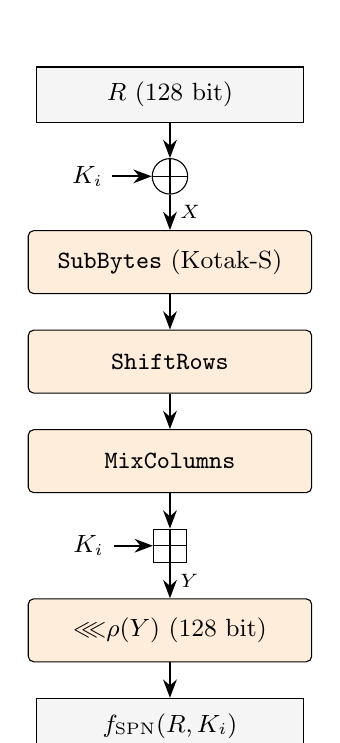
\begin{tikzpicture}[node distance=0.45cm, font=\small]
            \node[data, minimum width=3.4cm] (in) {$R$ (128 bit)};
            \node[xorop, below=of in] (x) {};
            \node[left=0.5cm of x] (k) {$K_i$};
            \node[blokspn, below=of x, minimum width=3.6cm] (sb) {\code{SubBytes} (Kotak-S)};
            \node[blokspn, below=of sb, minimum width=3.6cm] (sr) {\code{ShiftRows}};
            \node[blokspn, below=of sr, minimum width=3.6cm] (mc) {\code{MixColumns}};
            \node[addop, below=of mc] (add) {};
            \node[left=0.5cm of add] (k2) {$K_i$};
            \node[blokspn, below=of add, minimum width=3.6cm] (rot) {$\rotl \rho(Y)$ (128 bit)};
            \node[data, below=of rot, minimum width=3.4cm] (out) {$f_{\text{SPN}}(R, K_i)$};
            \draw[panah] (in) -- (x);
            \draw[panah] (k) -- (x);
            \draw[panah] (x) -- node[right, font=\scriptsize] {$X$} (sb);
            \draw[panah] (sb) -- (sr);
            \draw[panah] (sr) -- (mc);
            \draw[panah] (mc) -- (add);
            \draw[panah] (k2) -- (add);
            \draw[panah] (add) -- node[right, font=\scriptsize] {$Y$} (rot);
            \draw[panah] (rot) -- (out);
        \end{tikzpicture}
        \caption{Fungsi ronde $f_{\text{SPN}}$ (ronde 2--17)}
        \label{fig:fspn}
    \end{subfigure}
    \caption{Dua jenis fungsi ronde pada \algname}
    \label{fig:fungsi-ronde}
\end{figure}

\subsection{Implementasi Game of Life Secara Bit-Paralel}
Setiap baris grid disimpan sebagai satu bilangan bulat (\textit{bitmask}), sehingga satu generasi GoL dihitung per baris dengan operasi bitwise, bukan per sel. Untuk baris $r$, delapan tetangga diperoleh dari baris di atas, baris itu sendiri, dan baris di bawahnya (indeks modulo jumlah baris), masing-masing dalam versi asli serta versi yang dirotasi satu bit ke kiri dan ke kanan. Rotasi ini mewujudkan batas toroidal pada arah horizontal.

Kedelapan \textit{bitmask} tetangga dijumlahkan secara paralel untuk 16 sel sekaligus menggunakan pohon penjumlah ala Wallace \cite{wallace1964} (\cref{fig:wallace}). Hasilnya berupa tiga \textit{bitmask}: $c_0$ (bit ke-0 jumlah tetangga), $c_1$ (bit ke-1), dan $c_{\ge4}$ (jumlah tetangga $\geq 4$). Aturan B3/S23 kemudian cukup dihitung dengan
\begin{equation}
    s' = \underbrace{(c_1 \wedge \lnot c_{\ge 4})}_{N \in \{2,3\}} \wedge (c_0 \vee s),
\end{equation}
yang secara aljabar sama dengan $(N = 3) \vee (s \wedge N \in \{2,3\})$.

\begin{figure}[H]
    \centering
    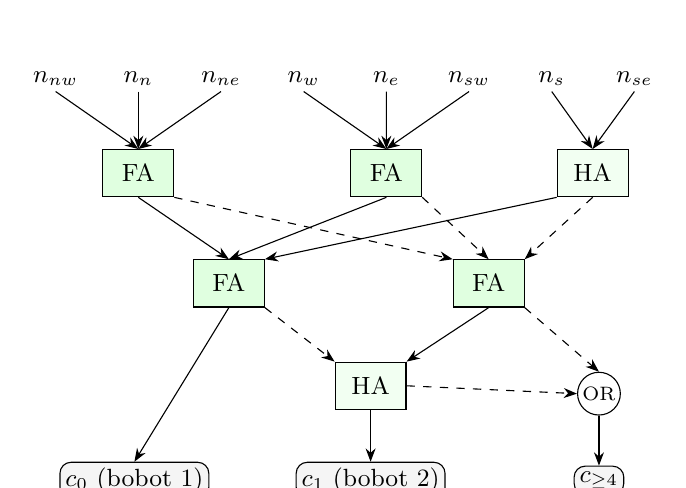
\begin{tikzpicture}[font=\small, every node/.style={inner sep=2pt},
        fa/.style={rectangle, draw, fill=green!12, minimum width=0.9cm, minimum height=0.6cm},
        ha/.style={rectangle, draw, fill=green!5, minimum width=0.9cm, minimum height=0.6cm}]
        \foreach \i/\n in {0/{nw},1/n,2/{ne},3/w,4/e,5/{sw},6/s,7/{se}} {
            \node (n\i) at (\i*1.05, 0) {$n_{\n}$};
        }
        \node[fa] (fa1) at (1.05,-1.2) {FA};
        \node[fa] (fa2) at (4.2,-1.2) {FA};
        \node[ha] (ha1) at (6.82,-1.2) {HA};
        \foreach \i in {0,1,2} \draw[-Stealth] (n\i.south) -- (fa1.north);
        \foreach \i in {3,4,5} \draw[-Stealth] (n\i.south) -- (fa2.north);
        \foreach \i in {6,7} \draw[-Stealth] (n\i.south) -- (ha1.north);

        \node[fa] (fa3) at (2.2,-2.6) {FA};
        \node[fa] (fa4) at (5.5,-2.6) {FA};
        \draw[-Stealth] (fa1.south) -- (fa3.north);
        \draw[-Stealth] (fa2.south) -- (fa3.north);
        \draw[-Stealth] (ha1.south west) -- (fa3.north east);
        \draw[-Stealth, dashed] (fa1.south east) -- (fa4.north west);
        \draw[-Stealth, dashed] (fa2.south east) -- (fa4.north);
        \draw[-Stealth, dashed] (ha1.south) -- (fa4.north east);

        \node[ha] (ha2) at (4.0,-3.9) {HA};
        \draw[-Stealth, dashed] (fa3.south east) -- (ha2.north west);
        \draw[-Stealth] (fa4.south) -- (ha2.north east);

        \node[draw, rounded corners, fill=gray!8] (c0) at (1.0,-5.1) {$c_0$ (bobot 1)};
        \node[draw, rounded corners, fill=gray!8] (c1) at (4.0,-5.1) {$c_1$ (bobot 2)};
        \node[circle, draw, inner sep=1pt, font=\scriptsize] (or) at (6.9,-4.0) {OR};
        \node[draw, rounded corners, fill=gray!8] (c4) at (6.9,-5.1) {$c_{\ge4}$};
        \draw[-Stealth] (fa3.south) -- (c0.north);
        \draw[-Stealth] (ha2.south) -- (c1.north);
        \draw[-Stealth, dashed] (fa4.south east) -- (or.north);
        \draw[-Stealth, dashed] (ha2.east) -- (or.west);
        \draw[-Stealth] (or.south) -- (c4.north);
    \end{tikzpicture}
    \caption{Pohon penjumlah untuk menghitung jumlah tetangga 16 sel sekaligus (FA = \textit{full adder}, HA = \textit{half adder}; garis putus-putus = \textit{carry})}
    \label{fig:wallace}
\end{figure}

\section{Fungsi Ronde \texorpdfstring{$f_{\text{SPN}}$}{f-SPN}}
\label{sec:fspn}
Fungsi ronde SPN didefinisikan sebagai
\begin{align}
    X &= R \oplus K, \nonumber\\
    Y &= \mathrm{MixColumns}\big(\mathrm{ShiftRows}(\mathrm{SubBytes}(X))\big) \boxplus K, \label{eq:fspn}\\
    f_{\text{SPN}}(R, K) &= Y \rotl \rho(Y), \qquad \rho(Y) = \big((5 \cdot y_0 + y_{15}) \oplus y_8\big) \bmod 128, \nonumber
\end{align}
dengan $y_j$ byte ke-$j$ dari $Y$ dan rotasi dilakukan pada $Y$ sebagai bilangan 128 bit \textit{big-endian}. Alurnya ditunjukkan pada \cref{fig:fspn}.

\subsection{Susunan State}
Sebanyak 16 byte $X = x_0 x_1 \dots x_{15}$ disusun menjadi matriks $4 \times 4$ \textbf{baris demi baris}. Susunan ini berbeda dengan AES yang mengisi \textit{state} kolom demi kolom. Akibatnya, \code{ShiftRows} menggeser byte yang berurutan di dalam masukan, sedangkan \code{MixColumns} mencampur byte yang berjarak 4 posisi (lihat \cref{tab:shiftrows}).

\subsection{Kotak-S (SubBytes)}
Setiap byte disubstitusi dengan Kotak-S AES (\cref{tab:sbox}). Kotak-S ini dipilih setelah iterasi desain. Versi awal rancangan kami menggunakan Kotak-S afin $S(x) = (167x + 91) \bmod 256$, tetapi analisis pada \cref{sec:iterasi-sbox} menunjukkan bahwa Kotak-S afin meloloskan selisih \code{0x80} dengan peluang 1. Kotak-S AES memiliki keseragaman diferensial 4 dan bias linear maksimum 16/256. Kedua nilai ini merupakan yang terbaik yang diketahui untuk permutasi 8 bit.

\begin{table}[H]
    \centering
    \caption{Kotak-S $8 \times 8$ bit yang dipakai pada $f_{\text{SPN}}$ (nilai heksadesimal; baris = 4 bit atas, kolom = 4 bit bawah masukan)}
    \label{tab:sbox}
    \footnotesize
    \setlength{\tabcolsep}{4.2pt}
    \ttfamily
    \begin{tabular}{c|cccccccccccccccc}
        \toprule
        & \textbf{0} & \textbf{1} & \textbf{2} & \textbf{3} & \textbf{4} & \textbf{5} & \textbf{6} & \textbf{7} & \textbf{8} & \textbf{9} & \textbf{A} & \textbf{B} & \textbf{C} & \textbf{D} & \textbf{E} & \textbf{F} \\
        \midrule
        \textbf{0} & 63 & 7c & 77 & 7b & f2 & 6b & 6f & c5 & 30 & 01 & 67 & 2b & fe & d7 & ab & 76 \\
        \textbf{1} & ca & 82 & c9 & 7d & fa & 59 & 47 & f0 & ad & d4 & a2 & af & 9c & a4 & 72 & c0 \\
        \textbf{2} & b7 & fd & 93 & 26 & 36 & 3f & f7 & cc & 34 & a5 & e5 & f1 & 71 & d8 & 31 & 15 \\
        \textbf{3} & 04 & c7 & 23 & c3 & 18 & 96 & 05 & 9a & 07 & 12 & 80 & e2 & eb & 27 & b2 & 75 \\
        \textbf{4} & 09 & 83 & 2c & 1a & 1b & 6e & 5a & a0 & 52 & 3b & d6 & b3 & 29 & e3 & 2f & 84 \\
        \textbf{5} & 53 & d1 & 00 & ed & 20 & fc & b1 & 5b & 6a & cb & be & 39 & 4a & 4c & 58 & cf \\
        \textbf{6} & d0 & ef & aa & fb & 43 & 4d & 33 & 85 & 45 & f9 & 02 & 7f & 50 & 3c & 9f & a8 \\
        \textbf{7} & 51 & a3 & 40 & 8f & 92 & 9d & 38 & f5 & bc & b6 & da & 21 & 10 & ff & f3 & d2 \\
        \textbf{8} & cd & 0c & 13 & ec & 5f & 97 & 44 & 17 & c4 & a7 & 7e & 3d & 64 & 5d & 19 & 73 \\
        \textbf{9} & 60 & 81 & 4f & dc & 22 & 2a & 90 & 88 & 46 & ee & b8 & 14 & de & 5e & 0b & db \\
        \textbf{A} & e0 & 32 & 3a & 0a & 49 & 06 & 24 & 5c & c2 & d3 & ac & 62 & 91 & 95 & e4 & 79 \\
        \textbf{B} & e7 & c8 & 37 & 6d & 8d & d5 & 4e & a9 & 6c & 56 & f4 & ea & 65 & 7a & ae & 08 \\
        \textbf{C} & ba & 78 & 25 & 2e & 1c & a6 & b4 & c6 & e8 & dd & 74 & 1f & 4b & bd & 8b & 8a \\
        \textbf{D} & 70 & 3e & b5 & 66 & 48 & 03 & f6 & 0e & 61 & 35 & 57 & b9 & 86 & c1 & 1d & 9e \\
        \textbf{E} & e1 & f8 & 98 & 11 & 69 & d9 & 8e & 94 & 9b & 1e & 87 & e9 & ce & 55 & 28 & df \\
        \textbf{F} & 8c & a1 & 89 & 0d & bf & e6 & 42 & 68 & 41 & 99 & 2d & 0f & b0 & 54 & bb & 16 \\
        \bottomrule
    \end{tabular}
\end{table}


\subsection{ShiftRows dan MixColumns}
\code{ShiftRows} merotasi baris ke-$i$ ($i = 0,1,2,3$) ke kiri sejauh $i$ byte (\cref{tab:shiftrows}). \code{MixColumns} mengalikan setiap kolom $(a_0, a_1, a_2, a_3)^T$ dengan matriks MDS AES di GF($2^8$):
\begin{equation}
    \begin{bmatrix} b_0 \\ b_1 \\ b_2 \\ b_3 \end{bmatrix} =
    \begin{bmatrix} 02 & 03 & 01 & 01 \\ 01 & 02 & 03 & 01 \\ 01 & 01 & 02 & 03 \\ 03 & 01 & 01 & 02 \end{bmatrix}
    \begin{bmatrix} a_0 \\ a_1 \\ a_2 \\ a_3 \end{bmatrix},
\end{equation}
dengan perkalian $02 \cdot a = (a \ll 1) \oplus (\texttt{0x1B} \text{ jika bit 7 } a = 1)$ dan $03 \cdot a = (02 \cdot a) \oplus a$. Kedua tabel perkalian ini dihitung di awal sebagai tabel \textit{lookup}.

\begin{table}[H]
    \centering
    \caption{Susunan \textit{state} $4\times4$ sebelum dan sesudah \code{ShiftRows} (indeks byte masukan)}
    \label{tab:shiftrows}
    \begin{tabular}{cccc c cccc}
        \multicolumn{4}{c}{\textbf{Sebelum}} & \quad & \multicolumn{4}{c}{\textbf{Sesudah}} \\
        \cmidrule{1-4} \cmidrule{6-9}
        $x_0$ & $x_1$ & $x_2$ & $x_3$ & & $x_0$ & $x_1$ & $x_2$ & $x_3$ \\
        $x_4$ & $x_5$ & $x_6$ & $x_7$ & $\xrightarrow{\;\ll 1\;}$ & $x_5$ & $x_6$ & $x_7$ & $x_4$ \\
        $x_8$ & $x_9$ & $x_{10}$ & $x_{11}$ & $\xrightarrow{\;\ll 2\;}$ & $x_{10}$ & $x_{11}$ & $x_8$ & $x_9$ \\
        $x_{12}$ & $x_{13}$ & $x_{14}$ & $x_{15}$ & $\xrightarrow{\;\ll 3\;}$ & $x_{15}$ & $x_{12}$ & $x_{13}$ & $x_{14}$ \\
    \end{tabular}
\end{table}

\subsection{Penjumlahan Modular dan Rotasi Bergantung Data}
Setelah \code{MixColumns}, \textit{state} dijumlahkan dengan \textit{round key} per byte modulo 256 ($\boxplus$). Kunci dengan demikian masuk dua kali ke $f_{\text{SPN}}$ melalui dua operasi dari struktur aljabar yang berbeda: XOR (penjumlahan di GF(2)) dan penjumlahan bilangan bulat modulo 256. Pencampuran kedua operasi ini, seperti pada IDEA dan RC6 \cite{rivest1998}, mempersulit analisis yang hanya bekerja di satu struktur aljabar.

Langkah terakhir adalah rotasi kiri 128 bit sejauh $\rho(Y) \in [0, 127]$ yang dihitung dari tiga byte $Y$ sendiri. Ide ini diambil dari RC5/RC6. Karena besar rotasi bergantung pada data, penyerang tidak dapat memprediksi posisi bit keluaran tanpa mengetahui nilai antara. Rotasi juga memindahkan bit melintasi batas byte, sehingga melengkapi \code{MixColumns} yang hanya bekerja di dalam kolom.

\section{Penjadwalan Kunci (Round Key)}
\label{sec:keysched}
Penjadwalan kunci menurunkan 18 \textit{round key} 128 bit dari kunci $K$ dan \textit{nonce} $N$. Gagasan utamanya adalah menjadikan kunci sebagai konfigurasi awal Game of Life, lalu mengambil \textit{round key} dari hasil evolusinya setelah di-\textit{whitening}. Alur lengkapnya ditunjukkan pada \cref{fig:keysched}.

\begin{figure}[H]
    \centering
    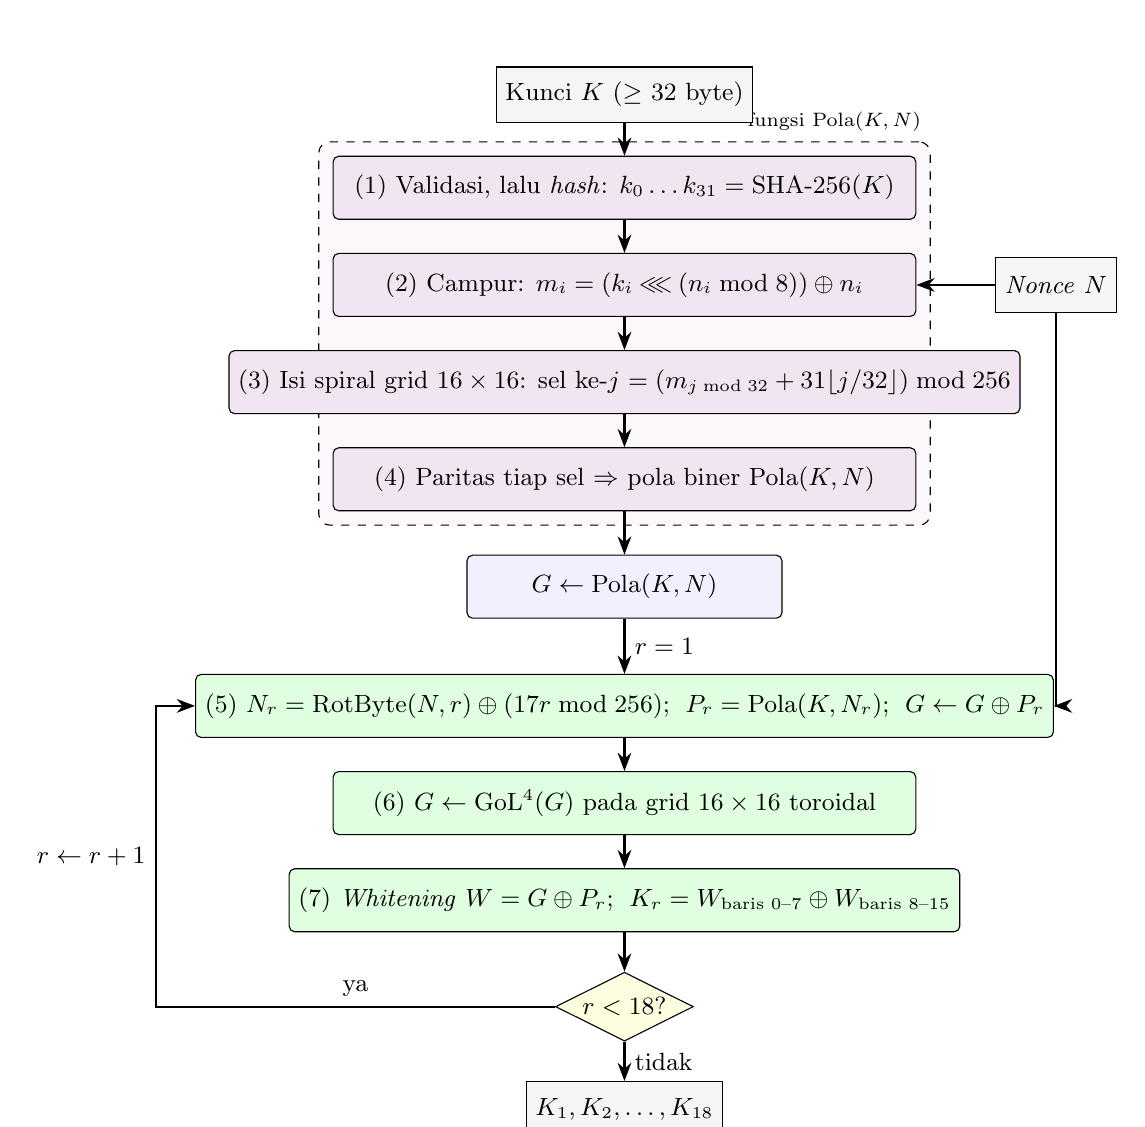
\begin{tikzpicture}[node distance=0.42cm, font=\small]
        \node[data] (k) {Kunci $K$ ($\geq$ 32 byte)};
        \node[blokkunci, below=of k, minimum width=7.4cm] (fold) {(1) Validasi, lalu \textit{hash}: $k_0 \dots k_{31} = \mathrm{SHA\text{-}256}(K)$};
        \node[blokkunci, below=of fold, minimum width=7.4cm] (mix) {(2) Campur: $m_i = (k_i \rotl (n_i \bmod 8)) \oplus n_i$};
        \node[blokkunci, below=of mix, minimum width=7.4cm] (spiral) {(3) Isi spiral grid $16\times16$: sel ke-$j$ $= (m_{j \bmod 32} + 31\lfloor j/32 \rfloor) \bmod 256$};
        \node[blokkunci, below=of spiral, minimum width=7.4cm] (par) {(4) Paritas tiap sel $\Rightarrow$ pola biner $\mathrm{Pola}(K, N)$};
        \node[blok, below=0.55cm of par, minimum width=4cm] (g0) {$G \leftarrow \mathrm{Pola}(K, N)$};

        \node[blokgol, below=0.7cm of g0, minimum width=7.4cm] (reinj) {(5) $N_r = \mathrm{RotByte}(N, r) \oplus (17r \bmod 256)$;\; $P_r = \mathrm{Pola}(K, N_r)$;\; $G \leftarrow G \oplus P_r$};
        \node[blokgol, below=of reinj, minimum width=7.4cm] (evo) {(6) $G \leftarrow \mathrm{GoL}^4(G)$ pada grid $16 \times 16$ toroidal};
        \node[blokgol, below=of evo, minimum width=7.4cm] (rk) {(7) \textit{Whitening} $W = G \oplus P_r$;\; $K_r = W_{\text{baris }0\text{--}7} \oplus W_{\text{baris }8\text{--}15}$};
        \node[keputusan, below=0.5cm of rk] (cek) {$r < 18$?};
        \node[data, below=0.5cm of cek] (out) {$K_1, K_2, \dots, K_{18}$};

        \node[data, right=1.0cm of mix] (n) {\textit{Nonce} $N$};

        \draw[panah] (k) -- (fold);
        \draw[panah] (fold) -- (mix);
        \draw[panah] (mix) -- (spiral);
        \draw[panah] (spiral) -- (par);
        \draw[panah] (par) -- (g0);
        \draw[panah] (g0) -- node[right] {$r = 1$} (reinj);
        \draw[panah] (reinj) -- (evo);
        \draw[panah] (evo) -- (rk);
        \draw[panah] (rk) -- (cek);
        \draw[panah] (cek) -- node[right] {tidak} (out);
        \draw[panah] (cek.west) -- node[above] {ya} ($(cek.west -| reinj.west)+(-0.5,0)$) |- node[pos=0.25, left] {$r \leftarrow r+1$} (reinj.west);
        \draw[panah] (n) -- (mix);
        \draw[panah] (n.south) |- (reinj.east);

        \begin{scope}[on background layer]
            \node[draw, dashed, rounded corners, fill=violet!3, fit=(fold)(par), inner sep=5pt, label={[font=\scriptsize, anchor=south east]north east:fungsi $\mathrm{Pola}(K, N)$}] {};
        \end{scope}
    \end{tikzpicture}
    \caption{Alur penjadwalan kunci berbasis Game of Life}
    \label{fig:keysched}
\end{figure}

Rincian setiap langkahnya adalah sebagai berikut.
\begin{enumerate}
    \item \textbf{Validasi dan \textit{hashing}.} Kunci minimal 32 byte (256 bit). Kunci sepanjang apa pun di-\textit{hash} dengan SHA-256 menjadi 32 byte $k_0, \dots, k_{31}$, sehingga setiap byte kunci memengaruhi seluruh materi kunci dan tidak ada dua kunci berbeda yang (secara praktis) menghasilkan materi yang sama.
    \item \textbf{Pencampuran dengan \textit{nonce}.} Setiap byte kunci dirotasi kiri 8 bit sejauh $n_i \bmod 8$, lalu di-XOR dengan $n_i$ (byte \textit{nonce} ke-$i$). Untuk \textit{nonce} tetap, langkah ini merupakan bijeksi pada setiap byte.
    \item \textbf{Pengisian spiral.} Ke-32 byte $m_i$ diisikan ke grid $16 \times 16$ mengikuti spiral searah jarum jam dari pojok kiri atas ke pusat (\cref{fig:spiral}). Karena grid memiliki 256 sel, materi 32 byte berulang sebanyak 8 putaran. Pada putaran ke-$\ell$ ($\ell = 0, \dots, 7$), nilainya ditambah $31\ell$ modulo 256 agar setiap putaran tidak sekadar menyalin putaran sebelumnya.
    \item \textbf{Paritas.} Setiap sel diganti dengan paritas jumlah bit 1-nya ($\mathrm{popcount} \bmod 2$), sehingga diperoleh grid biner $16 \times 16$ (256 bit) dengan kepadatan sel hidup sekitar 0,5.
    \item \textbf{Injeksi ulang \textit{nonce}.} Pada ronde ke-$r$, \textit{nonce} dirotasi sejauh $r$ byte dan setiap byte-nya di-XOR dengan $17r \bmod 256$. Pola baru $\mathrm{Pola}(K, N_r)$ dihitung dengan langkah 1--4, lalu di-XOR ke grid. Injeksi ulang mencegah grid mati atau terjebak pada pola periodik (osilator atau \textit{still life}), sehingga setiap ronde menerima entropi baru dari kunci.
    \item \textbf{Evolusi.} Grid dievolusikan 4 generasi Game of Life pada grid toroidal $16 \times 16$.
    \item \textbf{\textit{Whitening} dan pelipatan.} Grid hasil evolusi di-XOR sekali lagi dengan pola injeksi $P_r$ dari langkah 5, menghasilkan $W = G \oplus P_r$. Grid 256 bit $W$ kemudian dilipat menjadi \textit{round key} 128 bit dengan meng-XOR-kan 8 baris atas dengan 8 baris bawah. Langkah \textit{whitening} ini menyeimbangkan proporsi bit 1 pada \textit{round key} (\cref{sec:rk-density}). Grid yang dibawa ke ronde berikutnya tetap $G$ (hasil evolusi tanpa \textit{whitening}).
\end{enumerate}

\begin{figure}[H]
    \centering
    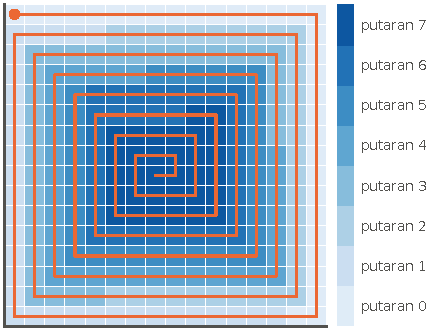
\includegraphics[width=0.42\textwidth]{spiral.pdf}
    \caption{Urutan pengisian spiral grid $16 \times 16$. Garis oranye menunjukkan urutan sel, dan warna menunjukkan putaran materi kunci ke-$\ell$ (32 sel per putaran).}
    \label{fig:spiral}
\end{figure}

\Cref{fig:ks-stages} menunjukkan contoh nyata tahapan penjadwalan kunci untuk kunci \code{"kunci-\allowbreak rahasia-\allowbreak minimal-\allowbreak 32-byte!!!"} dengan \textit{nonce} $N = \mathrm{SHA\text{-}256}(\texttt{"IF4020"})$. \textit{Round key} pertama yang dihasilkan adalah
\begin{center}
    $K_1 = $ \code{f9ec878321d2537857cb46413165e4f2}.
\end{center}

\begin{figure}[H]
    \centering
    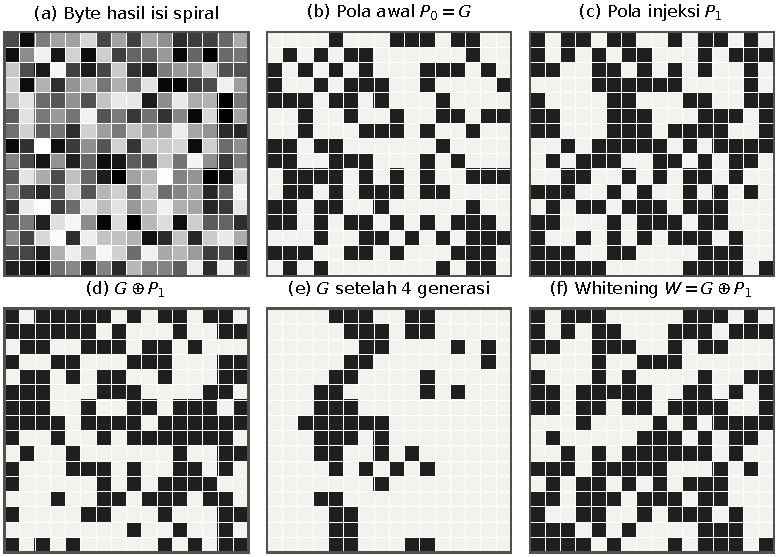
\includegraphics[width=0.86\textwidth]{ks_stages.pdf}
    \caption{Contoh tahapan penjadwalan kunci pada ronde pertama. Sel hitam bernilai 1 (hidup); panel (a) menampilkan nilai byte 0--255 dalam skala abu-abu. Panel (f) adalah grid yang dilipat menjadi $K_1$.}
    \label{fig:ks-stages}
\end{figure}

\section{Dekripsi}
\label{sec:dekripsi}
Karena memakai struktur Feistel, dekripsi blok menggunakan prosedur yang sama dengan enkripsi, tetapi \textit{round key} dipakai dengan urutan terbalik. Masukan $C$ dipecah menjadi $L'_0 \Vert R'_0 = R_{18} \Vert L_{18}$, lalu untuk $j = 1, \dots, 18$ dengan indeks kunci $i = 19 - j$:
\begin{equation}
    L'_j = R'_{j-1}, \qquad R'_j = L'_{j-1} \oplus F_i(R'_{j-1}, K_i).
\end{equation}
Jenis fungsi ronde mengikuti indeks kunci $i$, bukan urutan eksekusi $j$. Dengan demikian, ronde dekripsi pertama memakai $f_{\text{GoL}}$ dengan $K_{18}$, dan ronde terakhir memakai $f_{\text{GoL}}$ dengan $K_1$ (\cref{tab:urutan-dekripsi}). Kebenaran dekripsi dapat ditunjukkan dengan induksi. Pada ronde pertama, $R'_1 = R_{18} \oplus F_{18}(L_{18}, K_{18}) = R_{18} \oplus F_{18}(R_{17}, K_{18}) = L_{17}$ dan $L'_1 = R_{17}$. Pola yang sama berulang hingga $R'_{18} \Vert L'_{18}$ bernilai $L_0 \Vert R_0 = P$. Pembuktian ini tidak memerlukan $f_{\text{GoL}}$ maupun $f_{\text{SPN}}$ untuk dapat dibalik.

\begin{table}[H]
    \centering
    \caption{Urutan ronde pada enkripsi dan dekripsi}
    \label{tab:urutan-dekripsi}
    \begin{tabular}{c cc c cc}
        \toprule
        \multirow{2}{*}{\textbf{Urutan}} & \multicolumn{2}{c}{\textbf{Enkripsi}} & & \multicolumn{2}{c}{\textbf{Dekripsi}} \\
        \cmidrule{2-3} \cmidrule{5-6}
        & Kunci & Fungsi & & Kunci & Fungsi \\
        \midrule
        1 & $K_1$ & $f_{\text{GoL}}$ & & $K_{18}$ & $f_{\text{GoL}}$ \\
        2 & $K_2$ & $f_{\text{SPN}}$ & & $K_{17}$ & $f_{\text{SPN}}$ \\
        $\vdots$ & $\vdots$ & $\vdots$ & & $\vdots$ & $\vdots$ \\
        17 & $K_{17}$ & $f_{\text{SPN}}$ & & $K_2$ & $f_{\text{SPN}}$ \\
        18 & $K_{18}$ & $f_{\text{GoL}}$ & & $K_1$ & $f_{\text{GoL}}$ \\
        \bottomrule
    \end{tabular}
\end{table}

\section{Mode Operasi}
\label{sec:mode}
\algname{} mendukung lima mode operasi standar \cite{sp80038a} dengan ukuran blok penuh 256 bit (\cref{tab:mode}). \textit{Nonce} berperan ganda. Pada semua mode, \textit{nonce} dipakai dalam penjadwalan kunci. Pada mode selain ECB, \textit{nonce} juga menjadi IV atau nilai awal \textit{counter}. Pemakaian ganda ini aman karena \textit{nonce} dibangkitkan secara acak untuk setiap pesan, dan IV memang tidak perlu dirahasiakan.

\begin{table}[H]
    \centering
    \caption{Mode operasi yang didukung ($E$/$D$ = enkripsi/dekripsi satu blok, $C_0 = O_0 = N$)}
    \label{tab:mode}
    \small
    \begin{tabularx}{\textwidth}{l l l Y}
        \toprule
        \textbf{Mode} & \textbf{Enkripsi} & \textbf{Dekripsi} & \textbf{Keterangan} \\
        \midrule
        ECB & $C_i = E(P_i)$ & $P_i = D(C_i)$ & Blok identik dalam satu pesan menghasilkan \textit{ciphertext} identik \\
        CBC & $C_i = E(P_i \oplus C_{i-1})$ & $P_i = D(C_i) \oplus C_{i-1}$ & Mode bawaan \\
        CFB & $C_i = P_i \oplus E(C_{i-1})$ & $P_i = C_i \oplus E(C_{i-1})$ & CFB blok penuh (256 bit), hanya memakai $E$ \\
        OFB & $O_i = E(O_{i-1}),\ C_i = P_i \oplus O_i$ & sama dengan enkripsi & Aliran kunci tidak bergantung pada pesan \\
        CTR & $C_i = P_i \oplus E(N + i - 1)$ & sama dengan enkripsi & $N$ dibaca sebagai bilangan bulat 256 bit \textit{big-endian} \\
        \bottomrule
    \end{tabularx}
\end{table}

\section{Padding dan Format Ciphertext}
\label{sec:padding}
\textit{Padding} PKCS\#7 diterapkan pada semua mode dengan ukuran blok 32 byte: sebanyak $p = 32 - (|P| \bmod 32)$ byte bernilai $p$ ditambahkan, dengan $1 \le p \le 32$. Pesan yang panjangnya tepat kelipatan 32 tetap mendapat satu blok \textit{padding} penuh (32 byte bernilai \code{0x20}), sehingga \textit{padding} selalu dapat dibuang tanpa ambiguitas. Saat dekripsi, \textit{padding} divalidasi: nilai $p$ harus berada di rentang 1--32 dan $p$ byte terakhir harus semuanya bernilai $p$. Jika tidak, dekripsi gagal dengan \code{ValueError}. Format keluaran akhirnya ditunjukkan pada \cref{fig:format}.

\begin{figure}[H]
    \centering
    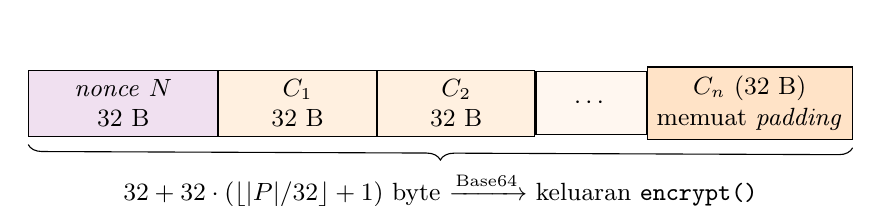
\begin{tikzpicture}[font=\small, cell/.style={draw, minimum height=0.8cm, align=center}]
        \node[cell, fill=violet!12, minimum width=2.4cm] (n) at (0,0) {\textit{nonce} $N$\\32 B};
        \node[cell, fill=orange!12, minimum width=2.0cm, right=0pt of n] (c1) {$C_1$\\32 B};
        \node[cell, fill=orange!12, minimum width=2.0cm, right=0pt of c1] (c2) {$C_2$\\32 B};
        \node[cell, fill=orange!6, minimum width=1.4cm, right=0pt of c2] (cd) {$\cdots$};
        \node[cell, fill=orange!22, minimum width=2.6cm, right=0pt of cd] (cn) {$C_n$ (32 B)\\memuat \textit{padding}};
        \draw[decorate, decoration={brace, amplitude=5pt, mirror}] ($(n.south west)+(0,-0.1)$) -- ($(cn.south east)+(0,-0.1)$) node[midway, below=6pt] {$32 + 32 \cdot (\lfloor |P|/32 \rfloor + 1)$ byte $\xrightarrow{\text{Base64}}$ keluaran \code{encrypt()}};
    \end{tikzpicture}
    \caption{Format \textit{ciphertext} \algname}
    \label{fig:format}
\end{figure}

\chapter{Implementasi dan Simulasi}
\label{ch:implementasi}

\section{Lingkungan dan Struktur Program}
\algname{} diimplementasikan dalam Python 3.13 tanpa pustaka kriptografi eksternal. Fungsi enkripsi dan dekripsi hanya memakai pustaka standar (\code{secrets} untuk \textit{nonce}, \code{hashlib} untuk SHA-256 pada penjadwalan kunci, dan \code{base64} untuk pengodean keluaran). Pustaka \code{numpy} dan \code{matplotlib} hanya dipakai oleh modul analisis. Struktur modulnya ditunjukkan pada \cref{tab:modul}.

\begin{table}[H]
    \centering
    \caption{Struktur modul pada paket \code{src}}
    \label{tab:modul}
    \small
    \begin{tabularx}{\textwidth}{l Y}
        \toprule
        \textbf{Modul} & \textbf{Tanggung jawab} \\
        \midrule
        \code{encrypt.py}, \code{decrypt.py} & Antarmuka utama \code{encrypt()} dan \code{decrypt()} \\
        \code{keygen.py} & Validasi dan \textit{hashing} kunci, pembangkitan \textit{nonce}, pengisian spiral, paritas, \textit{whitening}, dan penurunan 18 \textit{round key} \\
        \code{automaton.py} & Game of Life bit-paralel pada grid toroidal (pohon penjumlah, aturan B3/S23) \\
        \code{feistel.py} & Jaringan Feistel 18 ronde, pemilihan fungsi ronde, dan $f_{\text{GoL}}$ \\
        \code{spn.py} & $f_{\text{SPN}}$: Kotak-S, \code{ShiftRows}, \code{MixColumns}, penjumlahan modular, rotasi bergantung data \\
        \code{modes.py} & Mode operasi ECB, CBC, CFB, OFB, dan CTR \\
        \code{padding.py} & \textit{Padding} PKCS\#7 dan validasinya \\
        \code{types.py} & Tipe data \code{Grid} (setiap baris disimpan sebagai \textit{bitmask} bilangan bulat) \\
        \code{analysis.py} & Uji \textit{avalanche}, entropi, dan histogram \\
        \bottomrule
    \end{tabularx}
\end{table}

\section{Antarmuka Program}
\algname{} disediakan sebagai pustaka Python dengan dua fungsi utama:
\begin{itemize}
    \item \code{encrypt(data, key, mode="CBC") -> bytes}: menerima \textit{plaintext} berupa \code{str}, \code{bytes}, atau \code{bytearray} (teks maupun isi berkas biner) dan mengembalikan Base64 dari $N \Vert C$;
    \item \code{decrypt(data, key, mode="CBC") -> bytes}: menerima keluaran \code{encrypt()} dan mengembalikan \textit{plaintext} asli dalam bentuk \code{bytes}.
\end{itemize}
Contoh pemakaian untuk teks dan berkas biner ditunjukkan pada \cref{lst:contoh}.

\noindent\begin{minipage}{\linewidth}
\begin{lstlisting}[language=Python, caption={Contoh pemakaian \code{encrypt()} dan \code{decrypt()}}, label={lst:contoh}]
from src.encrypt import encrypt
from src.decrypt import decrypt

key = "kunci-rahasia-minimal-32-byte!!!"           # 32 byte
ct = encrypt("Halo, dunia!", key, mode="CTR")      # bytes Base64
assert decrypt(ct, key, mode="CTR") == b"Halo, dunia!"

with open("test/berkas/image.jpg", "rb") as f:     # berkas biner
    data = f.read()
ct = encrypt(data, key, mode="OFB")
assert decrypt(ct, key, mode="OFB") == data
\end{lstlisting}
\end{minipage}

Pustaka ini didistribusikan melalui halaman \textit{Releases} di GitHub. Setiap kali ada perubahan di \textit{branch} \code{main}, GitHub Actions otomatis membuat rilis baru berisi arsip \code{pregnant\_sister-vX.Y.Z.zip} (dan \code{.tar.gz}). Arsip ini memuat seluruh isi repositori: kode pustaka (\code{src}), \code{requirements.txt}, \textit{test} beserta berkas ujinya, laporan, dan dokumentasi API. Pengguna cukup mengekstrak arsip, menjalankan \code{pip install -r requirements.txt}, lalu mengimpor \code{src.encrypt} dan \code{src.decrypt} atau menjalankan skrip pengujian dari akar arsip.

Dokumentasi API lengkap dipublikasikan di \url{https://cola1000.github.io/Pregnant_Sister/} (\cref{fig:api}). Dokumentasi ini memuat cara instalasi dari rilis, parameter dan tipe data kedua fungsi, format \textit{ciphertext}, mode operasi, contoh penggunaan, penanganan galat, serta catatan keamanan.

\begin{figure}[H]
    \centering
    \fbox{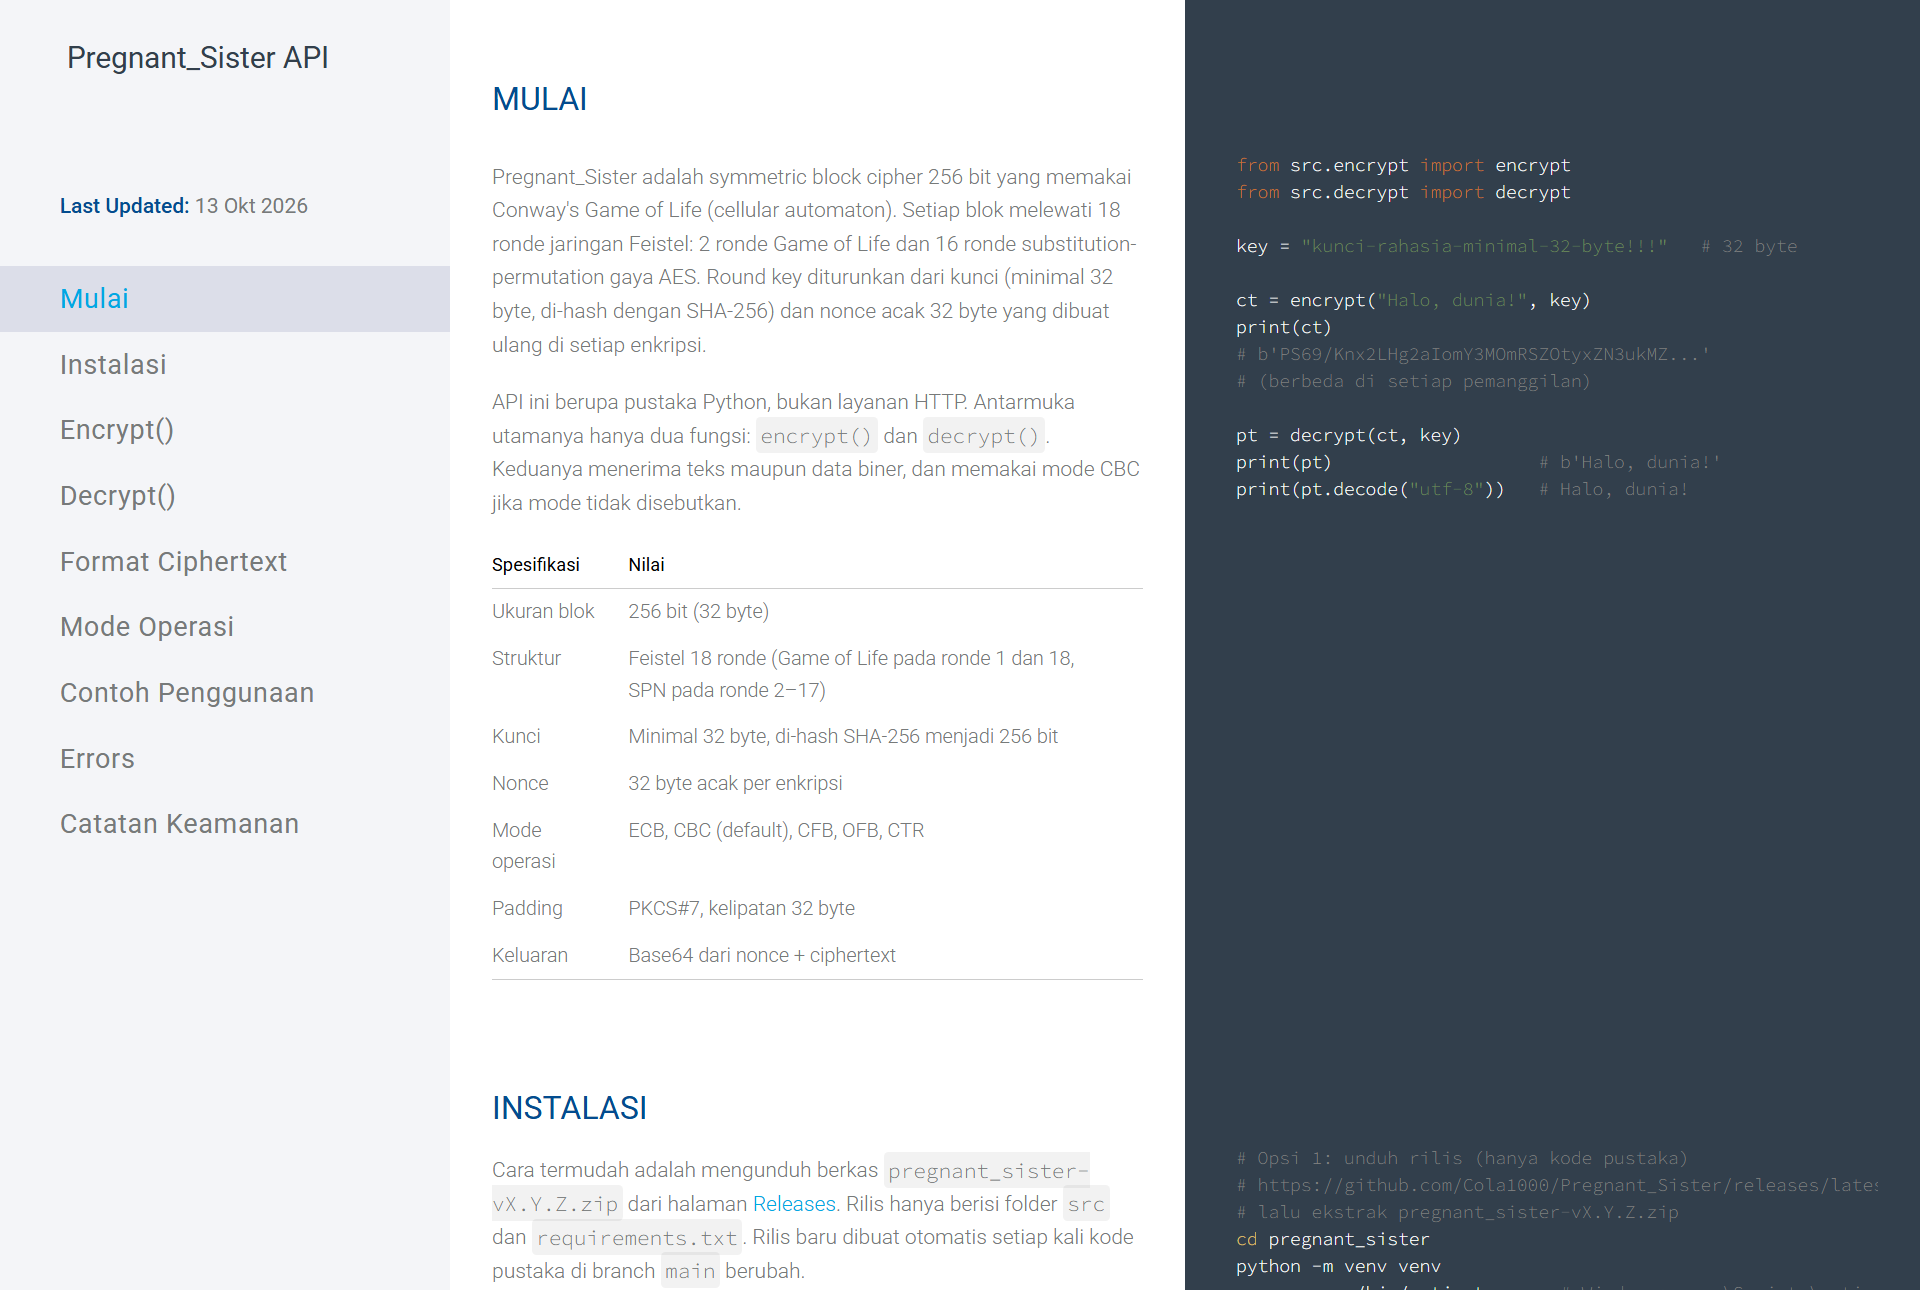
\includegraphics[width=0.92\textwidth]{api_docs.png}}
    \caption{Halaman dokumentasi API \algname}
    \label{fig:api}
\end{figure}

Selain pustaka, repositori menyediakan skrip pengujian yang dijalankan dari direktori akar (\cref{lst:skrip}).

\noindent\begin{minipage}{\linewidth}
\begin{lstlisting}[language=bash, caption={Skrip pengujian yang tersedia}, label={lst:skrip}]
python -m test.test_text        # analisis berkas teks (CBC)
python -m test.test_image       # analisis berkas gambar (CBC)
python -m test.test_video       # analisis berkas video (CBC)
python -m test.test_encrypt     # round-trip lima mode untuk semua berkas
python -m test.test_security    # evaluasi keamanan (Bab 5)
python -m test.test_keygen      # unit test penjadwalan kunci
python -m test.test_automaton   # unit test Game of Life
\end{lstlisting}
\end{minipage}

\section{Skenario Pengujian}
Pengujian dilakukan pada tiga berkas di \code{test/berkas} (\cref{tab:berkas}) dengan kunci 35 byte \code{"000\ldots0"} (35 karakter \code{'0'}). Kunci ini sengaja dipilih berpola agar terlihat bahwa \textit{ciphertext} tetap tampak acak walaupun kuncinya lemah secara visual. Berkas teks dan citra diuji pada kelima mode, sedangkan berkas video diuji pada mode CBC. Untuk setiap pengujian, kami mencatat ukuran \textit{ciphertext}, waktu enkripsi dan dekripsi, serta \textit{hash} SHA-256 dari \textit{plaintext} asli dan hasil dekripsi. Seluruh pengujian dijalankan pada mesin pengembang (Windows 11, Python 3.13.7).

\begin{table}[H]
    \centering
    \caption{Berkas uji}
    \label{tab:berkas}
    \begin{tabular}{l l r}
        \toprule
        \textbf{Berkas} & \textbf{Jenis} & \textbf{Ukuran (byte)} \\
        \midrule
        \code{glasses.txt} & teks ASCII berbahasa Inggris & 1.032 \\
        \code{image.jpg} & biner (citra JPEG) & 833.290 \\
        \code{video.mp4} & biner (video MP4) & 39.228.657 \\
        \bottomrule
    \end{tabular}
\end{table}

\section{Hasil Enkripsi dan Dekripsi}

\subsection{Berkas Teks}
\Cref{tab:hasil-teks} menunjukkan bahwa kelima mode mengembalikan berkas teks secara utuh. \textit{Ciphertext} mentah berukuran 1.088 byte, yaitu 32 byte \textit{nonce} ditambah 1.056 byte data (1.032 byte \textit{plaintext} ditambah 24 byte \textit{padding}). Walaupun \textit{plaintext} dan kuncinya sama, awalan \textit{ciphertext} berbeda pada setiap mode dan setiap eksekusi karena \textit{nonce} dibangkitkan secara acak.

\begin{table}[H]
    \centering
    \caption{Hasil enkripsi--dekripsi \code{glasses.txt} (SHA-256 \textit{plaintext} = \code{76d3bcab876abc41\ldots})}
    \label{tab:hasil-teks}
    \small\setlength{\tabcolsep}{4pt}
    \begin{tabular}{l r r r l c}
        \toprule
        \textbf{Mode} & \textbf{Mentah (B)} & \textbf{Base64 (B)} & \textbf{Enk + Dek (s)} & \textbf{Awalan Base64} & \textbf{SHA-256 sama} \\
        \midrule
        ECB & 1.088 & 1.452 & 0,02 + 0,02 & \code{FausVPMQ6FdvselD\ldots} & \checkmark \\
        CBC & 1.088 & 1.452 & 0,02 + 0,02 & \code{TMbd8jBi5LTpdZ4/\ldots} & \checkmark \\
        CFB & 1.088 & 1.452 & 0,02 + 0,02 & \code{FfINU8zWIv2+NQvq\ldots} & \checkmark \\
        OFB & 1.088 & 1.452 & 0,02 + 0,02 & \code{zpFhCn8xRThkoAne\ldots} & \checkmark \\
        CTR & 1.088 & 1.452 & 0,03 + 0,03 & \code{s4IBPE0rgSBj4nmc\ldots} & \checkmark \\
        \bottomrule
    \end{tabular}
\end{table}

\subsection{Berkas Biner}
\Cref{tab:hasil-biner} menunjukkan hasil untuk berkas citra JPEG. Kelima mode kembali mengembalikan berkas secara utuh, dan berkas hasil dekripsi dapat dibuka kembali sebagai gambar yang identik dengan aslinya. Waktu proses sekitar 12--14 detik per arah, yang setara dengan laju sekitar 60--70 KB/s. Laju ini wajar untuk implementasi Python murni yang menjalankan 18 ronde Feistel per blok.

\begin{table}[H]
    \centering
    \caption{Hasil enkripsi--dekripsi \code{image.jpg} (SHA-256 \textit{plaintext} = \code{5a92b5ae1f92711d\ldots})}
    \label{tab:hasil-biner}
    \small\setlength{\tabcolsep}{4pt}
    \begin{tabular}{l r r r l c}
        \toprule
        \textbf{Mode} & \textbf{Mentah (B)} & \textbf{Base64 (B)} & \textbf{Enk + Dek (s)} & \textbf{Awalan Base64} & \textbf{SHA-256 sama} \\
        \midrule
        ECB & 833.344 & 1.111.128 & 12,38 + 14,23 & \code{omJYfWOjziOuq/N2\ldots} & \checkmark \\
        CBC & 833.344 & 1.111.128 & 11,83 + 12,07 & \code{OZKtQ6Sq7KdFkgfE\ldots} & \checkmark \\
        CFB & 833.344 & 1.111.128 & 11,99 + 11,81 & \code{ZrkGsc34edw8uSqx\ldots} & \checkmark \\
        OFB & 833.344 & 1.111.128 & 12,04 + 11,70 & \code{d8268e8ICcqGvbgH\ldots} & \checkmark \\
        CTR & 833.344 & 1.111.128 & 11,65 + 11,96 & \code{pW908tgQo8GVnHXq\ldots} & \checkmark \\
        \bottomrule
    \end{tabular}
\end{table}

Berkas video 39 MB hanya diuji dengan mode CBC, karena setiap arah membutuhkan sekitar 10 menit (\cref{tab:hasil-video}). Kebenaran kelima mode pada data biner sudah ditunjukkan oleh berkas citra. Skrip \code{test.test\_encrypt} tetap dapat dipakai untuk menguji video pada kelima mode, dengan waktu total sekitar 1,5 jam.

\begin{table}[H]
    \centering
    \caption{Hasil enkripsi--dekripsi \code{video.mp4} (SHA-256 \textit{plaintext} = \code{f8564e7de424642c\ldots})}
    \label{tab:hasil-video}
    \small\setlength{\tabcolsep}{4pt}
    \begin{tabular}{l r r r l c}
        \toprule
        \textbf{Mode} & \textbf{Mentah (B)} & \textbf{Base64 (B)} & \textbf{Enk + Dek (s)} & \textbf{Awalan Base64} & \textbf{SHA-256 sama} \\
        \midrule
        CBC & 39.228.704 & 52.304.940 & 594,45 + 563,29 & \code{3Li8Ac7JD1iAs7lM\ldots} & \checkmark \\
        \bottomrule
    \end{tabular}
\end{table}

\subsection{Enkripsi Probabilistik}
Mengenkripsi \textit{plaintext} \code{"Halo, dunia!"} dua kali dengan kunci dan mode yang sama menghasilkan dua \textit{ciphertext} yang sama sekali berbeda:
\begin{center}
    \code{sBYT/+P7ag6EmtcTZWO8guwS4HL5BWw8fa9oNjwaFlEZ\ldots} \\
    \code{oqGOzWvLxJ8o32eP/q0z4RkpiObsWrgvPF7z4Klit3SQ\ldots}
\end{center}
Kedua \textit{ciphertext} tetap terdekripsi menjadi \textit{plaintext} yang sama. Sifat ini mencegah penyerang mengetahui apakah dua pesan memiliki isi yang sama.

\section{Analisis Penanganan Padding}
\label{sec:analisis-padding}
\Cref{tab:padding} menunjukkan perilaku \textit{padding} pada panjang \textit{plaintext} di sekitar batas blok. Untuk setiap panjang, dilakukan \textit{round-trip} pada kelima mode, dan semuanya berhasil.

\begin{table}[H]
    \centering
    \caption{Perilaku \textit{padding} PKCS\#7 (blok 32 byte) pada berbagai panjang \textit{plaintext}}
    \label{tab:padding}
    \small
    \begin{tabular}{r r r l r c}
        \toprule
        \textbf{$|P|$ (B)} & \textbf{$p$} & \textbf{\shortstack{Setelah\\\textit{padding} (B)}} & \textbf{\shortstack{Byte terakhir\\(heks)}} & \textbf{\shortstack{Mentah +\\\textit{nonce} (B)}} & \textbf{\shortstack{\textit{Round-trip}\\5 mode}} \\
        \midrule
        0   & 32 & 32  & \code{20 20 20 \ldots\ 20} & 64  & \checkmark \\
        1   & 31 & 32  & \code{1f 1f 1f \ldots\ 1f} & 64  & \checkmark \\
        15  & 17 & 32  & \code{11 11 11 \ldots\ 11} & 64  & \checkmark \\
        31  & 1  & 32  & \code{01}                  & 64  & \checkmark \\
        32  & 32 & 64  & \code{20 20 20 \ldots\ 20} & 96  & \checkmark \\
        33  & 31 & 64  & \code{1f 1f 1f \ldots\ 1f} & 96  & \checkmark \\
        63  & 1  & 64  & \code{01}                  & 96  & \checkmark \\
        64  & 32 & 96  & \code{20 20 20 \ldots\ 20} & 128 & \checkmark \\
        100 & 28 & 128 & \code{1c 1c 1c \ldots\ 1c} & 160 & \checkmark \\
        \bottomrule
    \end{tabular}
\end{table}

Ada tiga hal penting dari hasil ini:
\begin{enumerate}
    \item \textbf{\textit{Padding} selalu ditambahkan.} \textit{Plaintext} kosong dan \textit{plaintext} yang panjangnya kelipatan 32 (0, 32, 64 byte) mendapat satu blok \textit{padding} penuh bernilai \code{0x20}. Tanpa aturan ini, \textit{plaintext} yang kebetulan berakhir dengan byte \code{0x01} tidak dapat dibedakan dari \textit{padding}.
    \item \textbf{\textit{Padding} juga dipakai pada mode aliran.} CFB, OFB, dan CTR sebenarnya tidak memerlukan \textit{padding}, tetapi rancangan kami tetap menerapkannya agar format \textit{ciphertext} seragam untuk semua mode. Konsekuensinya, \textit{ciphertext} selalu 1--32 byte lebih panjang dari \textit{plaintext}.
    \item \textbf{\textit{Padding} divalidasi saat dekripsi.} Fungsi \code{unpad} menolak nilai $p$ di luar rentang 1--32 dan $p$ byte terakhir yang tidak seragam. Validasi ini juga berfungsi sebagai pendeteksi kesalahan sederhana (\cref{sec:integritas}).
\end{enumerate}

\section{Verifikasi Integritas Data}
\label{sec:integritas}

\subsection{Kecocokan Hash}
Integritas hasil dekripsi diverifikasi dengan membandingkan \textit{hash} SHA-256 berkas asli dan berkas hasil dekripsi. Pada \cref{tab:hasil-teks,tab:hasil-biner,tab:hasil-video}, kesebelas pasangan berkas dan mode menghasilkan \textit{hash} yang identik, sehingga hasil dekripsi sama persis bit demi bit dengan berkas asli. \textit{Hash} lengkapnya dicantumkan pada \cref{app:hash}. Pengujian \code{test\_security} juga menjalankan \textit{round-trip} untuk panjang 0, 1, 31, 32, 33, dan 100 byte dengan kunci acak sepanjang 32--71 byte pada kelima mode, dan tidak ada satu pun kegagalan.

\subsection{Deteksi Kunci atau Mode yang Salah}
Validasi \textit{padding} memberikan deteksi kesalahan secara tidak langsung. Jika kunci salah, blok terakhir hasil dekripsi praktis acak, sehingga peluang \textit{padding}-nya kebetulan valid sekitar $\sum_{p=1}^{32} 2^{-8p} \approx 1/255$. Hasil eksperimen pada \cref{tab:deteksi} sesuai dengan perkiraan tersebut.

\begin{table}[H]
    \centering
    \caption{Deteksi dekripsi dengan kunci atau mode yang salah (400 percobaan per skenario)}
    \label{tab:deteksi}
    \begin{tabular}{l r r}
        \toprule
        \textbf{Skenario} & \textbf{Terdeteksi (\code{ValueError})} & \textbf{Lolos tanpa galat} \\
        \midrule
        Kunci salah, mode CBC & 399 & 1 \\
        Kunci salah, mode CTR & 397 & 3 \\
        Enkripsi CBC, dekripsi CTR & 399 & 1 \\
        \bottomrule
    \end{tabular}
\end{table}

\subsection{Deteksi Perubahan Ciphertext}
Untuk menguji apakah perubahan pada \textit{ciphertext} terdeteksi, kami membalik satu bit pada blok kedua \textit{ciphertext} sebuah pesan empat blok, lalu menghitung jumlah bit yang berubah pada setiap blok hasil dekripsi (\cref{tab:propagasi}). Kami juga membalik satu bit acak pada blok terakhir sebanyak 300 kali per mode.

\begin{table}[H]
    \centering
    \caption{Propagasi galat akibat pembalikan 1 bit pada blok \textit{ciphertext} $C_2$ (jumlah bit berubah dari 256 bit per blok \textit{plaintext})}
    \label{tab:propagasi}
    \begin{tabular}{l c c c c c c r}
        \toprule
        \textbf{Mode} & $P_1$ & $P_2$ & $P_3$ & $P_4$ & $P_5$ (\textit{pad}) & \textbf{Terdeteksi?} & \textbf{Ubah blok terakhir terdeteksi} \\
        \midrule
        ECB & 0 & 120 & 0 & 0 & 0 & tidak & 299/300 \\
        CBC & 0 & 130 & 1 & 0 & 0 & tidak & 298/300 \\
        CFB & 0 & 1 & 126 & 0 & 0 & tidak & 133/300 \\
        OFB & 0 & 1 & 0 & 0 & 0 & tidak & 125/300 \\
        CTR & 0 & 1 & 0 & 0 & 0 & tidak & 131/300 \\
        \bottomrule
    \end{tabular}
\end{table}

Hasil ini sesuai dengan teori mode operasi. Pada ECB dan CBC, blok yang diubah terdekripsi menjadi data acak, dan pada CBC satu bit yang sama juga ikut terbalik di blok berikutnya. Pada CFB terjadi kebalikannya: bit yang sama terbalik di blok tersebut, lalu blok berikutnya rusak. Pada OFB dan CTR, hanya bit yang sama di \textit{plaintext} yang terbalik. \textbf{Tidak satu pun perubahan di tengah pesan terdeteksi}, karena blok \textit{padding} tidak tersentuh.

Perubahan pada blok terakhir terdeteksi hampir selalu pada ECB/CBC (seluruh blok terakhir menjadi acak sehingga \textit{padding} rusak). Pada mode aliran, perubahan hanya terdeteksi jika bit yang dibalik jatuh di area \textit{padding} (14 dari 32 byte pada pesan ini, sekitar 44\%). Kesimpulannya, \textbf{validasi \textit{padding} bukan mekanisme integritas}. \algname{} memberikan kerahasiaan, tetapi tidak memberikan autentikasi pesan. Implikasi keamanannya dibahas pada \cref{sec:integritas-keamanan}.

\chapter{Analisis Keamanan}
\label{ch:analisis}

Bab ini membahas hasil pengujian \textit{avalanche effect}, entropi, dan histogram, lalu dilanjutkan dengan pengujian tambahan terhadap komponen rancangan. Pengujian tingkat blok dijalankan dengan \code{test/test\_security.py}, yang keluaran lengkapnya terdapat pada \cref{app:security}. Pengujian tingkat berkas memakai berkas dan kunci yang sama dengan \cref{ch:implementasi}.

\section{Avalanche Effect}

\subsection{Tingkat Blok}
Uji \textit{avalanche} paling bersih dilakukan pada satu blok dengan \textit{round key} tetap, agar pengaruh \textit{nonce} acak tidak ikut terhitung. Untuk 20 blok acak, setiap bit dari 256 bit \textit{plaintext} dibalik satu per satu (total 5.120 pasangan), lalu dihitung jarak Hamming antara kedua \textit{ciphertext}. Hal yang sama dilakukan untuk setiap bit kunci ke-4 (64 pasangan) dengan \textit{nonce} tetap. Hasilnya ditunjukkan pada \cref{tab:avalanche-blok}.

\begin{table}[H]
    \centering
    \caption{\textit{Avalanche effect} tingkat blok (256 bit)}
    \label{tab:avalanche-blok}
    \begin{tabular}{l r r r}
        \toprule
        \textbf{Perubahan 1 bit pada} & \textbf{Rata-rata} & \textbf{Minimum} & \textbf{Maksimum} \\
        \midrule
        \textit{Plaintext} & 49,95\% & 98 bit (38,3\%) & 162 bit (63,3\%) \\
        Kunci & 50,46\% & 115 bit (44,9\%) & -- \\
        \bottomrule
    \end{tabular}
\end{table}

Rata-rata keduanya sangat dekat dengan nilai ideal 50\%. Rentang 98--162 bit juga konsisten dengan distribusi binomial $\mathrm{B}(256, \tfrac12)$, yang memiliki simpangan baku 8 bit. Nilai ekstrem 98 dan 162 bit berjarak sekitar 3,8 dan 4,3 simpangan baku dari rata-rata 128. Dengan 5.120 sampel, peluang munculnya minimal satu nilai sejauh 4,3 simpangan baku secara kebetulan sekitar 10\%, sehingga hasil ini sesuai dengan perilaku permutasi acak.

\subsection{Difusi terhadap Jumlah Ronde}
Untuk melihat seberapa cepat difusi tercapai, \textit{avalanche} diukur ulang dengan hanya menjalankan $n$ ronde pertama, untuk $n = 1, \dots, 18$ (\cref{fig:difusi}). Difusi penuh (sekitar 50\%) tercapai setelah \textbf{4 ronde}. Hal ini sesuai dengan struktur Feistel: satu bit di $R_0$ memengaruhi seluruh $R_1$ melalui $F$, lalu membutuhkan satu ronde lagi untuk menyebar ke paruh lainnya. Dengan 18 ronde, \algname{} memiliki margin keamanan sekitar 4,5 kali jumlah ronde minimum untuk difusi penuh. Margin ini sebanding dengan AES-128, yang mencapai difusi penuh setelah 2 ronde dan memakai 10 ronde.

\begin{figure}[H]
    \centering
    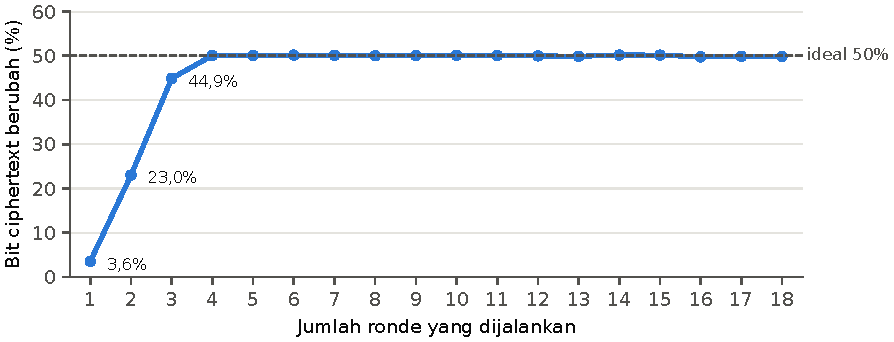
\includegraphics[width=\textwidth]{diffusion_rounds.pdf}
    \caption{Persentase bit \textit{ciphertext} yang berubah terhadap jumlah ronde yang dijalankan (12 blok $\times$ 64 posisi bit per titik)}
    \label{fig:difusi}
\end{figure}

\subsection{Tingkat Berkas pada Setiap Mode}
\Cref{tab:avalanche-mode} menunjukkan \textit{avalanche} pada 2.048 byte pertama setiap berkas (seluruh isi untuk \code{glasses.txt}). \textit{Nonce} yang sama dipakai untuk kedua enkripsi, dan bit yang dibalik adalah bit pertama \textit{plaintext} atau bit terakhir byte pertama kunci.

\begin{table}[H]
    \centering
    \caption{\textit{Avalanche effect} tingkat berkas per mode operasi}
    \label{tab:avalanche-mode}
    \begin{tabular}{l r r r r}
        \toprule
        \multirow{2}{*}{\textbf{Mode}} & \multicolumn{2}{c}{\textbf{1 bit \textit{plaintext}}} & \multicolumn{2}{c}{\textbf{1 bit kunci}} \\
        \cmidrule(lr){2-3} \cmidrule(lr){4-5}
        & \code{glasses.txt} & \code{image.jpg} & \code{glasses.txt} & \code{image.jpg} \\
        \midrule
        ECB & 1,46\% & 0,72\% & 50,27\% & 50,67\% \\
        CBC & 49,89\% & 49,87\% & 49,47\% & 50,52\% \\
        CFB & 48,88\% & 49,18\% & 50,39\% & 50,57\% \\
        OFB & 0,01\% & 0,01\% & 50,66\% & 50,79\% \\
        CTR & 0,01\% & 0,01\% & 50,79\% & 49,95\% \\
        \bottomrule
    \end{tabular}
\end{table}

Perubahan \textbf{kunci} menghasilkan \textit{avalanche} sekitar 50\% pada kelima mode, karena seluruh \textit{round key} ikut berubah. Sebaliknya, \textit{avalanche} terhadap perubahan \textbf{\textit{plaintext}} sangat bergantung pada mode:
\begin{itemize}
    \item \textbf{CBC dan CFB} (sekitar 50\%): perubahan pada blok pertama merambat ke semua blok berikutnya melalui rantai umpan balik.
    \item \textbf{ECB} (1,46\% dan 0,72\%): hanya blok pertama yang berubah, dan sekitar setengah bitnya berubah. Karena blok pertama hanya 1/33 dan 1/65 bagian dari data yang diukur (termasuk blok \textit{padding}), persentase totalnya kecil.
    \item \textbf{OFB dan CTR} (0,01\% = tepat 1 bit): aliran kunci tidak bergantung pada \textit{plaintext}, sehingga membalik satu bit \textit{plaintext} hanya membalik satu bit yang sama di \textit{ciphertext}.
\end{itemize}
Nilai kecil pada ECB, OFB, dan CTR \textbf{bukan kelemahan \textit{block cipher}}, melainkan sifat bawaan mode tersebut yang juga berlaku pada AES. Hasil tingkat blok pada \cref{tab:avalanche-blok} menunjukkan bahwa fungsi $E$ sendiri memiliki \textit{avalanche} yang ideal. Hal ini juga menjelaskan mengapa \code{src/analysis.py} memakai mode CBC untuk pengukuran \textit{avalanche}.

\section{Entropi}
Entropi Shannon dihitung pada \textit{ciphertext} mentah tanpa \textit{nonce}. Base64 tidak dipakai karena hanya memiliki 64 simbol, sehingga entropinya tidak mungkin melebihi 6 bit per byte. Hasilnya ditunjukkan pada \cref{tab:entropi}.

\begin{table}[H]
    \centering
    \caption{Entropi Shannon (bit per byte, maksimum 8) \textit{plaintext} dan \textit{ciphertext}}
    \label{tab:entropi}
    \begin{tabular}{l r r r r r r r}
        \toprule
        \multirow{2}{*}{\textbf{Berkas}} & \multirow{2}{*}{\textbf{\textit{Plaintext}}} & \multicolumn{5}{c}{\textbf{\textit{Ciphertext}}} & \multirow{2}{*}{\textbf{Harapan acak}} \\
        \cmidrule(lr){3-7}
        & & ECB & CBC & CFB & OFB & CTR & \\
        \midrule
        \code{glasses.txt} & 4,3935 & 7,7762 & 7,8292 & 7,8137 & 7,8386 & 7,8077 & 7,8258 \\
        \code{image.jpg}   & 7,9306 & 7,9997 & 7,9998 & 7,9998 & 7,9998 & 7,9998 & 7,9998 \\
        \code{video.mp4}   & 7,9993 & -- & 8,0000 & -- & -- & -- & 8,0000 \\
        64 KB byte nol     & 0,0000 & -- & 7,9973 & -- & -- & -- & 7,9972 \\
        \bottomrule
    \end{tabular}
\end{table}

Entropi \textit{ciphertext} \code{glasses.txt} (7,78--7,84) tampak lebih rendah daripada berkas lain, tetapi nilai ini memang yang diharapkan dari data acak sempurna berukuran sama. Entropi yang diukur dari sampel berhingga sebanyak $n$ byte bersifat bias ke bawah, dengan nilai harapan sekitar \cite{miller1955}
\begin{equation}
    \mathbb{E}[\hat{H}] \approx 8 - \frac{255}{2n \ln 2}.
\end{equation}
Untuk $n = 1.056$ byte, nilai harapannya 7,8258, sehingga hasil 7,78--7,84 sesuai dengan keluaran yang acak. Untuk citra ($n = 833.312$), nilai harapannya 7,9998, dan untuk video ($n = 39.228.672$) nilai harapannya 7,999995. Keduanya sama dengan hasil pengukuran. Video MP4 yang sudah terkompresi memiliki entropi \textit{plaintext} 7,9993, sehingga entropi saja tidak dapat membedakan \textit{plaintext} terkompresi dari \textit{ciphertext}. Karena itu, histogram dan uji $\chi^2$ pada subbab berikutnya tetap diperlukan. Kasus paling ekstrem adalah 64 KB byte nol (entropi \textit{plaintext} 0): \textit{ciphertext}-nya tetap mencapai entropi 7,9973. Artinya, keacakan keluaran tidak bergantung pada keacakan masukan.

\section{Histogram}
\Cref{fig:hist-teks,fig:hist-citra,fig:hist-video} membandingkan histogram nilai byte \textit{plaintext} dan \textit{ciphertext} (mode CBC). Histogram \textit{plaintext} teks terkonsentrasi pada rentang huruf ASCII (sekitar 97--122) dan spasi (32). Histogram citra JPEG tidak rata, dengan puncak paling menonjol di nilai \code{0x00} (sekitar 2,7 kali rata-rata). Setelah dienkripsi, kedua histogram menjadi rata di sekitar nilai harapan (garis putus-putus), tanpa sisa pola dari \textit{plaintext}.

\begin{figure}[H]
    \centering
    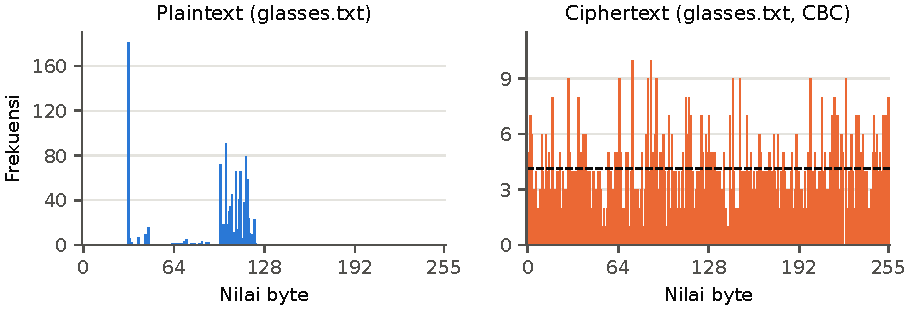
\includegraphics[width=\textwidth]{hist_text.pdf}
    \caption{Histogram \code{glasses.txt}: \textit{plaintext} (kiri) dan \textit{ciphertext} CBC (kanan). Garis putus-putus menunjukkan frekuensi harapan distribusi seragam.}
    \label{fig:hist-teks}
\end{figure}

\begin{figure}[H]
    \centering
    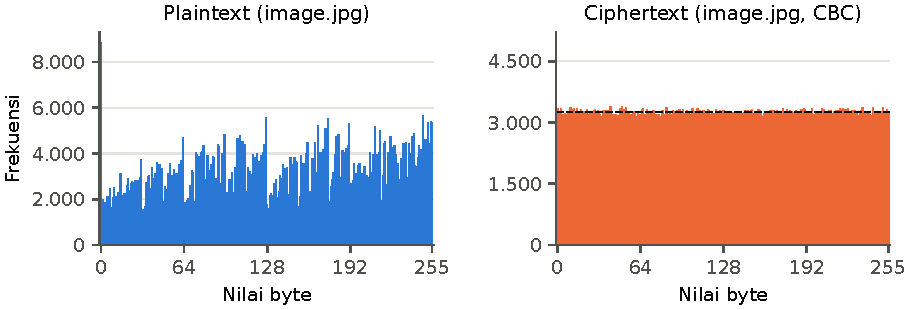
\includegraphics[width=\textwidth]{hist_image.pdf}
    \caption{Histogram \code{image.jpg}: \textit{plaintext} (kiri) dan \textit{ciphertext} CBC (kanan)}
    \label{fig:hist-citra}
\end{figure}

\begin{figure}[H]
    \centering
    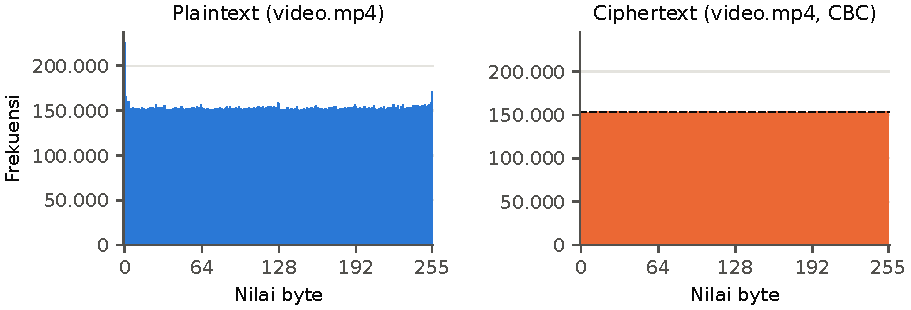
\includegraphics[width=\textwidth]{hist_video.pdf}
    \caption{Histogram \code{video.mp4}: \textit{plaintext} (kiri) dan \textit{ciphertext} CBC (kanan)}
    \label{fig:hist-video}
\end{figure}

Kerataan histogram diuji secara kuantitatif dengan uji $\chi^2$ (255 derajat kebebasan, nilai kritis 293,25 pada $\alpha = 5\%$). Hasilnya ditunjukkan pada \cref{tab:chi2}.

\begin{table}[H]
    \centering
    \caption{Statistik $\chi^2$ histogram (lolos jika $< 293{,}25$)}
    \label{tab:chi2}
    \begin{tabular}{l r r r r r r}
        \toprule
        \textbf{Berkas} & \textbf{\textit{Plaintext}} & \textbf{ECB} & \textbf{CBC} & \textbf{CFB} & \textbf{OFB} & \textbf{CTR} \\
        \midrule
        \code{glasses.txt} & 17.551 & 309,3$^{*}$ & 241,5 & 257,0 & 224,5 & 264,2 \\
        \code{image.jpg}   & 81.473 & 304,1$^{*}$ & 228,4 & 250,7 & 262,4 & 252,9 \\
        \code{video.mp4}   & 42.092 & -- & 252,4 & -- & -- & -- \\
        64 KB byte nol     & -- & -- & 239,6 & -- & -- & -- \\
        \bottomrule
    \end{tabular}
\end{table}

Seluruh \textit{ciphertext} pada mode CBC, CFB, OFB, dan CTR, serta \textit{ciphertext} video dan berkas nol, lolos uji $\chi^2$. Dua nilai pada mode ECB melewati batas: 309,3 pada berkas teks ($p \approx 0{,}011$) dan 304,1 pada citra ($p \approx 0{,}019$). ECB memang memetakan blok \textit{plaintext} identik ke blok \textit{ciphertext} identik, sehingga kami terlebih dahulu memeriksa apakah blok berulang menjadi penyebabnya. Ternyata \code{glasses.txt} tidak memiliki blok 32 byte yang berulang, dan \code{image.jpg} hanya memiliki 33 blok duplikat dari 26.040 blok, jumlah yang terlalu kecil untuk memengaruhi histogram. Karena itu, kami mengulang enkripsi berkas teks sebanyak 300 kali dengan \textit{nonce} berbeda untuk setiap mode, dan mengulang enkripsi ECB citra sebanyak 20 kali (\cref{tab:chi2-ulang}).

\begin{table}[H]
    \centering
    \caption{Distribusi $\chi^2$ dari enkripsi ulang dengan \textit{nonce} berbeda}
    \label{tab:chi2-ulang}
    \begin{tabular}{l r r r r}
        \toprule
        \textbf{Mode} & \textbf{Rata-rata} & \textbf{Simpangan baku} & \textbf{Melewati 293,25} & \textbf{Maksimum} \\
        \midrule
        \multicolumn{5}{l}{\textit{\code{glasses.txt}, 300 kali per mode}} \\
        ECB & 255,8 & 22,8 & 7,0\% & 314,7 \\
        CBC & 254,6 & 21,9 & 3,7\% & 331,6 \\
        CFB & 255,1 & 21,5 & 5,3\% & 333,1 \\
        OFB & 256,2 & 23,0 & 6,0\% & 323,4 \\
        CTR & 255,1 & 21,4 & 3,0\% & 341,8 \\
        \midrule
        \multicolumn{5}{l}{\textit{\code{image.jpg}, 20 kali}} \\
        ECB & 253,8 & 24,8 & 15\% (3 dari 20) & 300,7 \\
        \midrule
        Teoretis $\chi^2_{255}$ & 255,0 & 22,6 & 5,0\% & -- \\
        \bottomrule
    \end{tabular}
\end{table}

Pada kelima mode, rata-rata dan simpangan baku $\chi^2$ sesuai dengan distribusi teoretis $\chi^2_{255}$. Proporsi yang melewati batas (3,0--7,0\%) berada dalam sekitar 1,6 galat baku dari nilai nominal 5\% (galat baku $\pm 1{,}3\%$ untuk 300 percobaan). Pada citra, 3 dari 20 percobaan ECB melewati batas, tetapi peluang mendapatkan minimal 3 kegagalan dari 20 percobaan secara kebetulan sekitar 7,5\%, dan rata-ratanya (253,8) tetap sesuai harapan. Enkripsi CTR atas 1 MB byte nol juga menghasilkan $\chi^2 = 238{,}8$. Dengan demikian, kegagalan pada \cref{tab:chi2} merupakan fluktuasi acak, bukan bias pada mode tertentu.

\section{Pengujian Tambahan}

\subsection{Kebocoran Pola pada Mode ECB}
Kelemahan klasik ECB diuji dengan citra mentah berukuran $256 \times 256$ piksel \textit{grayscale} (1 byte per piksel) yang memiliki banyak area seragam (\cref{fig:ecb}). Citra ini memiliki 2.048 blok, tetapi hanya 270 blok yang berbeda. Pada ECB, \textit{ciphertext}-nya juga memiliki tepat 270 blok berbeda, sehingga bentuk-bentuk pada citra masih terlihat jelas. Pada CBC dan CTR, ke-2.048 blok \textit{ciphertext} semuanya berbeda dan citra tampak seperti derau. Percobaan dengan 100 blok \textit{plaintext} identik menunjukkan hal yang sama: ECB hanya menghasilkan 2 blok \textit{ciphertext} berbeda, yaitu blok data dan blok \textit{padding}.

\begin{figure}[H]
    \centering
    \begin{subfigure}{0.23\textwidth}\centering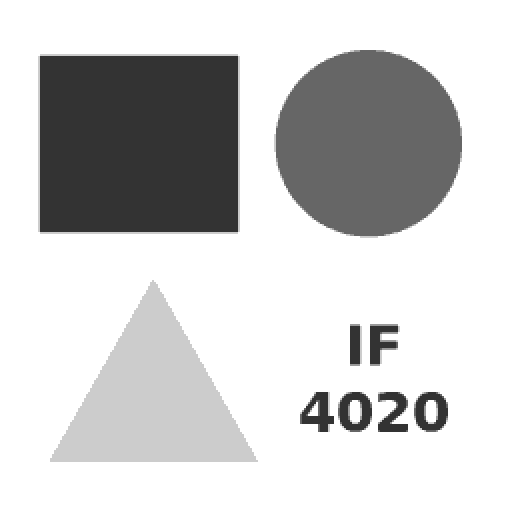
\includegraphics[width=\linewidth]{ecb_plain.png}\caption{\textit{Plaintext}}\end{subfigure}\hfill
    \begin{subfigure}{0.23\textwidth}\centering
\includegraphics[width=\linewidth]{ecb_ecb.png}\caption{ECB}\end{subfigure}\hfill
    \begin{subfigure}{0.23\textwidth}\centering
\includegraphics[width=\linewidth]{ecb_cbc.png}\caption{CBC}\end{subfigure}\hfill
    \begin{subfigure}{0.23\textwidth}\centering
\includegraphics[width=\linewidth]{ecb_ctr.png}\caption{CTR}\end{subfigure}
    \caption{Citra mentah yang dienkripsi dengan ECB, CBC, dan CTR (setiap baris citra 256 piksel = 8 blok)}
    \label{fig:ecb}
\end{figure}

\textit{Nonce} per pesan membuat \algname{} lebih baik daripada ECB pada AES dalam satu hal: blok yang sama pada \textbf{dua pesan berbeda} menghasilkan \textit{ciphertext} berbeda, karena \textit{round key}-nya berbeda. Namun, di \textbf{dalam satu pesan}, ECB tetap membocorkan pola, sehingga mode ini tidak disarankan untuk data berpola.

\subsection{Analisis Kotak-S dan Iterasi Desain}
\label{sec:iterasi-sbox}
Versi awal $f_{\text{SPN}}$ memakai Kotak-S afin $S(x) = (167x + 91) \bmod 256$. Analisis diferensial menunjukkan bahwa selisih $\Delta = \texttt{0x80}$ pada setiap byte lolos melalui seluruh komponen $f_{\text{SPN}}$:
\begin{itemize}
    \item \textbf{Kotak-S}: $x \oplus \texttt{0x80} = x + 128 \pmod{256}$, sehingga $S(x \oplus \texttt{0x80}) = S(x) + 167 \cdot 128 = S(x) + 128 = S(x) \oplus \texttt{0x80}$ (karena 167 ganjil). Peluangnya 1.
    \item \textbf{\code{MixColumns}}: jika keempat byte suatu kolom memiliki selisih \code{0x80}, selisih keluarannya adalah $(02 \oplus 03 \oplus 01 \oplus 01) \cdot \texttt{0x80} = \texttt{0x80}$. Peluangnya 1.
    \item \textbf{Penjumlahan mod 256}: selisih \code{0x80} hanya mengenai bit paling signifikan, sehingga tidak menghasilkan \textit{carry}. Peluangnya 1.
    \item \textbf{Rotasi}: besar rotasi $\rho$ tidak berubah, karena bit 7 dihapus oleh $\bmod\ 128$, dan pola \code{0x80} berulang tetap terjaga jika $\rho \equiv 0 \pmod 8$. Peluangnya $2^{-3}$.
\end{itemize}
Akibatnya, setiap ronde SPN yang aktif hanya memberikan peluang $2^{-3}$. Ini adalah kelemahan fatal. Kotak-S kemudian diganti dengan Kotak-S AES. \Cref{tab:sbox-analisis} membandingkan kedua Kotak-S, dan pengujian ulang menunjukkan bahwa karakteristik \code{0x80} tidak pernah muncul lagi (0 dari 4.000 percobaan pada $f_{\text{SPN}}$ dan 0 dari 20.000 percobaan pada 6 ronde tereduksi).

\begin{table}[H]
    \centering
    \caption{Perbandingan Kotak-S versi awal dan versi akhir}
    \label{tab:sbox-analisis}
    \small
    \begin{tabularx}{\textwidth}{Y c c}
        \toprule
        \textbf{Sifat} & \textbf{Afin $(167x+91) \bmod 256$} & \textbf{AES (versi akhir)} \\
        \midrule
        Afin terhadap $\mathbb{Z}_{256}$ & ya & tidak \\
        Nilai maksimum DDT & 256/256 (untuk $\Delta = \texttt{0x80}$) & 4/256 \\
        Bias linear maksimum (LAT) & 128/256 (bit terendah linear) & 16/256 \\
        Peluang $\texttt{0x80..80} \to \texttt{0x80..80}$ pada $f_{\text{SPN}}$ & $2^{-3}$ & 0/4.000 (tidak teramati) \\
        \bottomrule
    \end{tabularx}
\end{table}

\subsection{Batas Kriptanalisis Diferensial}
Pada jaringan Feistel dengan fungsi ronde yang (hampir) bijektif, setiap tiga ronde berurutan memiliki minimal dua ronde aktif. Jika ronde $i$ tidak aktif ($\Delta R_{i-1} = 0$), maka $\Delta R_i = \Delta L_{i-1} \neq 0$ menjadi masukan ronde $i+1$, sedangkan $\Delta L_i = 0$. Masukan ronde $i+2$ adalah $\Delta R_{i+1} = \Delta L_i \oplus \Delta F_{i+1} = \Delta F_{i+1}$, yang tidak nol jika $F$ bijektif. Dari 16 ronde SPN, minimal 10 ronde aktif. Setiap $f_{\text{SPN}}$ yang aktif mengaktifkan minimal satu Kotak-S dengan peluang diferensial maksimum $2^{-6}$, sehingga peluang karakteristik diferensial apa pun dibatasi oleh
\begin{equation}
    p \le \left(2^{-6}\right)^{10} = 2^{-60}.
\end{equation}
Batas ini dapat dibuktikan, tetapi masih longgar. Batas ini belum mencapai $2^{-256}$ (ukuran blok), sehingga belum menjadi jaminan formal. Batas sebenarnya hampir pasti jauh lebih kecil, karena \code{MixColumns} dengan \textit{branch number} 5 umumnya mengaktifkan banyak Kotak-S pada ronde berikutnya, dan rotasi yang bergantung data mengacak posisi selisih. Skrip \code{test\_security} memberikan estimasi heuristik $\leq 2^{-132}$ untuk karakteristik iteratif 3 ronde, tetapi estimasi ini hanya berlaku untuk satu jenis karakteristik. Pembuktian batas yang ketat, misalnya dengan menghitung jumlah minimum Kotak-S aktif menggunakan MILP, menjadi salah satu saran pengembangan.

\subsection{Iterasi Desain Penjadwalan Kunci: Distribusi Bit Round Key}
\label{sec:rk-density}
Versi awal penjadwalan kunci mengambil \textit{round key} langsung dari lipatan grid hasil evolusi, yaitu $K_r = \mathrm{Lipat}(G)$. Pengukuran pada 300 pasangan kunci dan \textit{nonce} acak menunjukkan bahwa proporsi bit 1 pada \textit{round key} versi tersebut hanya \textbf{0,362}, bukan 0,5. Penyebabnya dapat dijelaskan dengan mengukur kepadatan grid pada setiap tahap:
\begin{enumerate}
    \item Setelah injeksi ulang, kepadatan grid sekitar 0,500, karena XOR dengan pola paritas yang seimbang mengembalikan grid ke keseimbangan.
    \item Empat generasi GoL menurunkan kepadatan menjadi sekitar $q = 0{,}237$, karena sel yang terlalu padat mati akibat \textit{overpopulation}. Penurunan ini adalah perilaku umum GoL pada konfigurasi acak.
    \item Pelipatan dengan XOR dua bit yang masing-masing bernilai 1 dengan peluang $q$ menghasilkan bit 1 dengan peluang $2q(1-q) = 2 \cdot 0{,}237 \cdot 0{,}763 = 0{,}362$, sesuai dengan hasil pengukuran.
\end{enumerate}
Jika bit-bitnya dianggap independen, entropi per bit \textit{round key} versi awal hanya $H(0{,}362) \approx 0{,}944$ bit, atau sekitar 120,9 bit per \textit{round key} 128 bit.

Versi akhir memperbaikinya dengan \textit{whitening}: sebelum dilipat, grid hasil evolusi di-XOR dengan pola injeksi $P_r$ dari ronde yang sama, sehingga $K_r = \mathrm{Lipat}(G \oplus P_r)$. Pola $P_r$ memiliki kepadatan sekitar 0,5, sehingga XOR dengannya menghapus bias yang ditimbulkan GoL. Grid yang dibawa ke ronde berikutnya tetap $G$, jadi dinamika GoL pada penjadwalan kunci tidak berubah; yang berubah hanya cara \textit{round key} diekstraksi. \Cref{fig:rk-density} membandingkan kedua versi.

\begin{figure}[H]
    \centering
    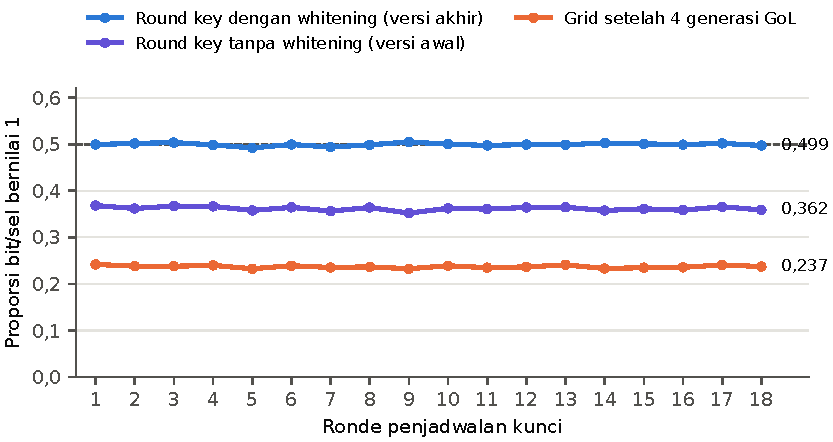
\includegraphics[width=\textwidth]{rk_density.pdf}
    \caption{Proporsi bit 1 pada grid dan \textit{round key} untuk setiap ronde penjadwalan kunci (300 pasangan kunci dan \textit{nonce} acak; angka di kanan = rata-rata 18 ronde; garis putus-putus = 0,5)}
    \label{fig:rk-density}
\end{figure}

Setelah \textit{whitening}, proporsi bit 1 menjadi \textbf{0,499}. Pengujian yang lebih rinci pada 54.000 \textit{round key} (3.000 pasangan kunci dan \textit{nonce} acak) menunjukkan bahwa masih tersisa bias kecil yang bergantung pada posisi bit. Proporsi per posisi berada di rentang 0,471--0,515, dan 3 dari 128 posisi menyimpang secara signifikan dari 0,5 ($|z| > 4$). Bit pada \textit{round key} yang berurutan tidak berkorelasi (koefisien korelasi 0,0001), sehingga bias ini bukan artefak sampel. Penyebabnya kemungkinan struktur spasial pengisian spiral, karena delapan sel yang berasal dari byte materi kunci yang sama saling berkorelasi. Dampaknya sangat kecil: jika setiap posisi dianggap independen, entropi \textit{round key} hanya berkurang sekitar 0,007 bit dari 128 bit. Entropi byte \textit{round key} juga mencapai 7,9981 dari 86.400 byte, sesuai dengan nilai harapan 7,9979 untuk data acak berukuran sama. Uji \code{test\_security} versi akhir juga melaporkan proporsi 0,4985 dan entropi byte 7,9934 (harapan 7,9936 untuk 28.800 byte) (\cref{app:security}).

Kami juga memeriksa apakah langkah paritas menghilangkan informasi kunci. Pada satu pola, setiap byte materi kunci (keluaran SHA-256 yang telah dicampur dengan \textit{nonce}) menentukan 8 bit paritas (satu untuk setiap putaran spiral), tetapi hanya ada 98 kombinasi yang berbeda dari 256 kemungkinan nilai byte (sekitar 6,3 bit informasi). Namun, jika ke-19 pola ($P_0$ dan 18 injeksi ulang dengan \textit{nonce} berbeda) digabungkan, ke-256 nilai setiap byte materi kunci dapat dibedakan pada 50 \textit{nonce} acak yang diuji. Dengan demikian, langkah paritas tidak menyempitkan ruang kunci di tingkat pola.

\subsection{Iterasi Desain Penjadwalan Kunci: Kunci Ekuivalen}
Versi awal melipat kunci yang lebih panjang dari 32 byte dengan XOR, sehingga kunci yang berbeda dapat menghasilkan materi kunci yang sama. Contoh ekstremnya, setiap kunci berbentuk $X \Vert X$ terlipat menjadi 32 byte nol. Pada versi tersebut, \textit{ciphertext} yang dienkripsi dengan kunci \code{"my secret key that is 32 bytes!!"} $\times 2$ dapat didekripsi dengan kunci \code{"A"} $\times 64$.

Versi akhir mengganti pelipatan dengan SHA-256. Karena SHA-256 tahan tabrakan, dua kunci berbeda praktis tidak mungkin menghasilkan materi kunci yang sama, dan setiap bit kunci memengaruhi seluruh 256 bit materi kunci. Pada versi akhir, dekripsi dengan kunci \code{"A"} $\times 64$ gagal dengan \code{ValueError} (\textit{padding} tidak valid), dan \code{test\_security} melaporkan bahwa kedua kunci tidak lagi saling menggantikan. Perlu dicatat bahwa SHA-256 adalah fungsi \textit{hash} yang cepat, bukan KDF untuk kata sandi. Jika kunci berasal dari frasa sandi berentropi rendah, KDF lambat dengan \textit{salt} tetap lebih tepat (\cref{sec:saran}).

\subsection{Integritas dan Malleability}
\label{sec:integritas-keamanan}
Seperti ditunjukkan pada \cref{tab:propagasi}, \algname{} tidak memiliki autentikasi pesan. Penyerang yang mengetahui sebagian isi \textit{plaintext} dapat mengubahnya secara terarah tanpa mengetahui kunci. Pada percobaan dengan mode CBC, membalik bit yang tepat di blok \textit{ciphertext} pertama mengubah \textit{plaintext} blok kedua dari \code{"PAY 0000100 USD\ldots"} menjadi \code{"PAY 9000100 USD\ldots"}, dan dekripsi tetap berhasil tanpa galat. Pada OFB dan CTR, manipulasi ini bahkan lebih mudah karena tidak ada blok yang rusak. Selain itu, fungsi \code{unpad} mengeluarkan dua pesan galat yang berbeda (\code{Invalid padding length} dan \code{Invalid padding sequence}). Jika pesan galat ini terlihat oleh penyerang, ia dapat dimanfaatkan sebagai \textit{padding oracle} pada mode CBC \cite{vaudenay2002}. Kedua masalah ini diatasi dengan skema \textit{Encrypt-then-MAC}, misalnya HMAC-SHA256 atas $N \Vert C$ dengan kunci terpisah \cite{bellare2000, rfc2104}.

\subsection{Kinerja}
Kinerja diukur pada mesin pengembang dengan Python 3.13 (\cref{tab:kinerja}). Penjadwalan kunci hanya dijalankan sekali per pesan, sehingga biaya utamanya adalah 18 ronde Feistel per blok. Laju sekitar 60--70 KB/s membuat implementasi ini cukup untuk berkas berukuran hingga beberapa MB, tetapi berkas 39 MB sudah membutuhkan hampir 10 menit per arah. Kinerja yang rendah ini sebagian besar disebabkan oleh interpretasi Python, bukan oleh rancangan algoritma. Operasi GoL bit-paralel, Kotak-S, dan \code{MixColumns} pada dasarnya hanya terdiri atas operasi bitwise dan \textit{lookup} tabel yang cepat di perangkat keras.

\begin{table}[H]
    \centering
    \caption{Hasil pengukuran kinerja}
    \label{tab:kinerja}
    \begin{tabular}{l r}
        \toprule
        \textbf{Operasi} & \textbf{Waktu / laju} \\
        \midrule
        Penjadwalan kunci (18 \textit{round key}) & 5,7 ms per pesan \\
        Enkripsi satu blok (32 byte) & 474 $\mu$s ($\approx$ 66 KB/s) \\
        Enkripsi / dekripsi \code{image.jpg} (833 KB) & $\approx$ 12 s ($\approx$ 68 KB/s) \\
        Enkripsi / dekripsi \code{video.mp4} (39,2 MB, CBC) & 594 s / 563 s ($\approx$ 64--68 KB/s) \\
        \bottomrule
    \end{tabular}
\end{table}

\section{Ringkasan Hasil Analisis}
\begin{table}[H]
    \centering
    \caption{Ringkasan hasil analisis keamanan}
    \label{tab:ringkasan}
    \small
    \begin{tabularx}{\textwidth}{l Y c}
        \toprule
        \textbf{Aspek} & \textbf{Hasil} & \textbf{Status} \\
        \midrule
        \textit{Round-trip} & teks dan citra pada 5 mode, video pada CBC, 9 panjang \textit{padding} pada 5 mode; \textit{hash} identik & baik \\
        \textit{Avalanche} \textit{plaintext}/kunci & 49,95\% / 50,46\% pada tingkat blok & baik \\
        Difusi & penuh setelah 4 dari 18 ronde & baik \\
        Entropi & sesuai harapan data acak pada semua ukuran & baik \\
        Histogram & rata; kegagalan $\chi^2$ yang sesekali muncul terbukti fluktuasi acak melalui pengujian berulang & baik \\
        Kotak-S & DDT 4/256, LAT 16/256 (setelah iterasi desain) & baik \\
        Batas diferensial terbukti & $\leq 2^{-60}$ (longgar) & perlu kajian \\
        Bit \textit{round key} & proporsi 0,499 setelah \textit{whitening} (sebelumnya 0,362); bias kecil per posisi, kehilangan entropi $\approx$ 0,007 bit & baik \\
        Derivasi kunci & SHA-256, tidak ada lagi kunci ekuivalen $X \Vert X$ & baik \\
        ECB & membocorkan pola di dalam satu pesan & sifat mode \\
        Integritas & tidak ada MAC; \textit{ciphertext} dapat dimanipulasi & lemah \\
        \bottomrule
    \end{tabularx}
\end{table}

\chapter{Kesimpulan dan Saran Pengembangan}
\label{ch:kesimpulan}

\section{Kesimpulan}
\begin{enumerate}
    \item Kami telah merancang \algname, sebuah \textit{block cipher} 256 bit berstruktur Feistel 18 ronde yang memadukan Conway's Game of Life dengan komponen SPN gaya AES. GoL dipakai di dua tempat: fungsi ronde $f_{\text{GoL}}$ pada ronde pertama dan terakhir, serta penjadwalan kunci yang menurunkan 18 \textit{round key} dari evolusi grid $16 \times 16$ dengan injeksi ulang \textit{nonce} dan \textit{whitening}. Struktur Feistel memungkinkan GoL, yang tidak dapat dibalik, dipakai sebagai fungsi ronde tanpa mengganggu proses dekripsi.
    \item Implementasi Python berhasil mengenkripsi dan mendekripsi berkas teks maupun biner pada kelima mode operasi (ECB, CBC, CFB, OFB, CTR). Seluruh hasil dekripsi identik bit demi bit dengan berkas asli, dibuktikan dengan kecocokan \textit{hash} SHA-256. \textit{Padding} PKCS\#7 menangani semua panjang pesan dengan benar, termasuk pesan kosong dan pesan yang panjangnya kelipatan ukuran blok.
    \item Secara statistik, \algname{} berperilaku seperti permutasi acak. \textit{Avalanche} terhadap \textit{plaintext} dan kunci masing-masing 49,95% dan 50,46%, difusi penuh tercapai setelah 4 dari 18 ronde, entropi \textit{ciphertext} sesuai dengan nilai harapan data acak pada setiap ukuran berkas, dan histogram \textit{ciphertext} rata, bahkan untuk \textit{plaintext} berupa byte nol. Kegagalan uji $\chi^2$ yang sesekali muncul terbukti sebagai fluktuasi acak melalui pengujian berulang.
    \item Analisis komponen menghasilkan tiga iterasi desain. Kotak-S afin pada versi awal meloloskan selisih \code{0x80} dengan peluang 1, sehingga diganti dengan Kotak-S AES. Pelipatan kunci dengan XOR membuat kunci $X \Vert X$ setara dengan kunci nol, sehingga diganti dengan SHA-256. \textit{Round key} yang diambil langsung dari grid hasil evolusi hanya memiliki proporsi bit 1 sebesar 0,362, sehingga ditambahkan \textit{whitening} yang menaikkannya menjadi 0,499. Temuan-temuan ini menunjukkan bahwa uji statistik seperti \textit{avalanche} dan entropi tidak cukup untuk menilai keamanan, karena versi awal pun lolos uji-uji tersebut.
    \item Beberapa keterbatasan masih tersisa pada versi akhir: \textit{ciphertext} tidak diautentikasi sehingga dapat dimanipulasi, batas peluang diferensial yang dapat dibuktikan baru $2^{-60}$, masih ada bias kecil yang bergantung pada posisi bit \textit{round key} (setara dengan kehilangan entropi sekitar 0,007 bit), dan kinerja implementasi Python hanya sekitar 60--70 KB/s.
\end{enumerate}

\section{Saran Pengembangan (Future Works)}
\label{sec:saran}
\begin{enumerate}
    \item \textbf{Autentikasi.} \textit{Encrypt-then-MAC} dengan HMAC-SHA256 atas $N \Vert C$ perlu ditambahkan, atau \algname{} dapat dikembangkan menjadi mode AEAD. Pesan galat \textit{padding} juga perlu disatukan agar tidak menjadi \textit{padding oracle}.
    \item \textbf{KDF untuk kata sandi.} SHA-256 sudah menghilangkan kunci ekuivalen, tetapi SHA-256 adalah fungsi \textit{hash} yang cepat. Untuk kunci yang berasal dari kata sandi, sebaiknya disediakan KDF lambat dengan \textit{salt}, seperti PBKDF2 atau Argon2, agar serangan tebakan kata sandi menjadi mahal.
    \item \textbf{Ekstraksi \textit{round key} yang lebih seragam.} Bias kecil per posisi bit dapat dihilangkan, misalnya dengan melewatkan grid hasil \textit{whitening} ke Kotak-S atau fungsi \textit{hash} sebelum dilipat, atau dengan mengacak urutan sel pada pengisian spiral.
    \item \textbf{Analisis formal.} Batas jumlah minimum Kotak-S aktif perlu dihitung dengan MILP untuk kriptanalisis diferensial dan linear. Kajian terhadap serangan \textit{related-key} juga perlu dilakukan, karena \textit{nonce} publik ikut menentukan \textit{round key}. Keluaran \textit{cipher} sebaiknya juga diuji dengan rangkaian uji statistik NIST SP 800-22 \cite{rukhin2010}.
    \item \textbf{Kinerja dan keamanan implementasi.} Laju sekitar 60--70 KB/s dapat ditingkatkan dengan implementasi bit-sliced dalam C/Rust atau dengan memproses blok secara paralel pada mode ECB dan CTR. Implementasi \textit{constant-time} juga diperlukan, karena \textit{lookup} Kotak-S dan rotasi dengan bilangan bulat Python berpotensi membocorkan informasi melalui waktu eksekusi.
    \item \textbf{Perbaikan antarmuka.} Mode operasi dapat disimpan di \textit{header ciphertext} agar penerima tidak perlu mengetahuinya terlebih dahulu. Galat validasi kunci sebaiknya dilempar sebagai \textit{exception}, bukan hanya dicetak. \textit{Counter} CTR juga perlu dibungkus modulo $2^{256}$ untuk menghindari \textit{overflow} pada \textit{nonce} yang sangat besar, walaupun peluang kejadiannya dapat diabaikan.
\end{enumerate}

\begin{thebibliography}{99}
\addcontentsline{toc}{chapter}{Daftar Pustaka}
\markboth{Daftar Pustaka}{Daftar Pustaka}

\bibitem{bellare2000}
M.~Bellare dan C.~Namprempre, ``Authenticated Encryption: Relations among Notions and Analysis of the Generic Composition Paradigm,'' dalam \textit{Advances in Cryptology -- ASIACRYPT 2000}, LNCS 1976. Springer, 2000, hlm.~531--545.

\bibitem{biham1991}
E.~Biham dan A.~Shamir, ``Differential Cryptanalysis of DES-like Cryptosystems,'' \textit{Journal of Cryptology}, vol.~4, no.~1, hlm.~3--72, 1991.

\bibitem{daemen2002}
J.~Daemen dan V.~Rijmen, \textit{The Design of Rijndael: AES -- The Advanced Encryption Standard}. Berlin: Springer, 2002.

\bibitem{sp80038a}
M.~Dworkin, ``Recommendation for Block Cipher Modes of Operation: Methods and Techniques,'' NIST Special Publication 800-38A, 2001.

\bibitem{feistel1973}
H.~Feistel, ``Cryptography and Computer Privacy,'' \textit{Scientific American}, vol.~228, no.~5, hlm.~15--23, 1973.

\bibitem{gardner1970}
M.~Gardner, ``Mathematical Games: The Fantastic Combinations of John Conway's New Solitaire Game `Life','' \textit{Scientific American}, vol.~223, no.~4, hlm.~120--123, 1970.

\bibitem{heys2002}
H.~M.~Heys, ``A Tutorial on Linear and Differential Cryptanalysis,'' \textit{Cryptologia}, vol.~26, no.~3, hlm.~189--221, 2002.

\bibitem{rfc5652}
R.~Housley, ``Cryptographic Message Syntax (CMS),'' RFC 5652, IETF, 2009.

\bibitem{rfc2104}
H.~Krawczyk, M.~Bellare, dan R.~Canetti, ``HMAC: Keyed-Hashing for Message Authentication,'' RFC 2104, IETF, 1997.

\bibitem{matsui1994}
M.~Matsui, ``Linear Cryptanalysis Method for DES Cipher,'' dalam \textit{Advances in Cryptology -- EUROCRYPT '93}, LNCS 765. Springer, 1994, hlm.~386--397.

\bibitem{miller1955}
G.~A.~Miller, ``Note on the Bias of Information Estimates,'' dalam H.~Quastler (ed.), \textit{Information Theory in Psychology: Problems and Methods}. Glencoe, IL: Free Press, 1955, hlm.~95--100.

\bibitem{munir2026}
R.~Munir, ``Block Cipher (Bagian 1),'' bahan kuliah IF4020 Kriptografi, Institut Teknologi Bandung, 2026. [Daring]. Tersedia: \url{https://informatika.stei.itb.ac.id/~rinaldi.munir/Kriptografi/2026-2027/08-Block-Cipher-Bagian1-(2026).pdf}

\bibitem{nandi1994}
S.~Nandi, B.~K.~Kar, dan P.~Pal~Chaudhuri, ``Theory and Applications of Cellular Automata in Cryptography,'' \textit{IEEE Transactions on Computers}, vol.~43, no.~12, hlm.~1346--1357, 1994.

\bibitem{fips46}
National Institute of Standards and Technology, ``Data Encryption Standard (DES),'' FIPS PUB 46-3, 1999.

\bibitem{fips197}
National Institute of Standards and Technology, ``Advanced Encryption Standard (AES),'' FIPS PUB 197, 2001.

\bibitem{rivest1998}
R.~L.~Rivest, M.~J.~B.~Robshaw, R.~Sidney, dan Y.~L.~Yin, ``The RC6 Block Cipher,'' proposal AES, 1998.

\bibitem{rukhin2010}
A.~Rukhin dkk., ``A Statistical Test Suite for Random and Pseudorandom Number Generators for Cryptographic Applications,'' NIST Special Publication 800-22 Rev.~1a, 2010.

\bibitem{shannon1948}
C.~E.~Shannon, ``A Mathematical Theory of Communication,'' \textit{Bell System Technical Journal}, vol.~27, no.~3, hlm.~379--423, 1948.

\bibitem{shannon1949}
C.~E.~Shannon, ``Communication Theory of Secrecy Systems,'' \textit{Bell System Technical Journal}, vol.~28, no.~4, hlm.~656--715, 1949.

\bibitem{vaudenay2002}
S.~Vaudenay, ``Security Flaws Induced by CBC Padding -- Applications to SSL, IPSEC, WTLS\ldots,'' dalam \textit{Advances in Cryptology -- EUROCRYPT 2002}, LNCS 2332. Springer, 2002, hlm.~534--545.

\bibitem{wallace1964}
C.~S.~Wallace, ``A Suggestion for a Fast Multiplier,'' \textit{IEEE Transactions on Electronic Computers}, vol.~EC-13, no.~1, hlm.~14--17, 1964.

\bibitem{webster1986}
A.~F.~Webster dan S.~E.~Tavares, ``On the Design of S-Boxes,'' dalam \textit{Advances in Cryptology -- CRYPTO '85}, LNCS 218. Springer, 1986, hlm.~523--534.

\bibitem{wolfram1986}
S.~Wolfram, ``Cryptography with Cellular Automata,'' dalam \textit{Advances in Cryptology -- CRYPTO '85}, LNCS 218. Springer, 1986, hlm.~429--432.

\end{thebibliography}


\appendix
\chapter{Tautan Repositori dan Dokumentasi}
\label{app:tautan}
\begin{itemize}
    \item Repositori kode sumber: \url{https://github.com/Cola1000/Pregnant_Sister}
    \item Dokumentasi API: \url{https://cola1000.github.io/Pregnant_Sister/}
\end{itemize}

\chapter{Keluaran Pengujian Keamanan}
\label{app:security}
Keluaran lengkap \code{python -m test.test\_security} (benih acak 69420) untuk versi akhir \algname{}. Semua pemeriksaan berlabel \code{[OK]}. Baris \textit{S-box is affine} bernilai \code{False} karena Kotak-S versi akhir bukan lagi Kotak-S afin, dan baris \textit{Keys X||X} menunjukkan bahwa kunci ekuivalen akibat pelipatan sudah tidak ada (\cref{ch:analisis}).

\begin{lstlisting}[numbers=none, basicstyle=\ttfamily\scriptsize, caption={Keluaran \code{test\_security}}]
[OK] Round-trip in all modes and lengths: 0 failures
[OK] Plaintext avalanche (block level): 49.95% (min 98, max 162 of 256 bits)
[OK] Key avalanche (block level): 50.46% (min 115 bits)
       full diffusion check, 2 rounds: 23.6%
       full diffusion check, 3 rounds: 45.0%
       full diffusion check, 4 rounds: 50.1%
[OK] Raw ciphertext of 64 KB zeros: entropy 7.9973/8, chi2 239.6 (df=255, pass < 293)
       note: base64 output can never exceed 6.0 bits entropy, so measure on raw bytes
       throughput: 68.3 KB/s
[OK] S-box is affine (167x + 91 mod 256): False
[OK] S-box max differential count: 4/256 (AES: 4/256)
[OK] S-box max linear bias: 16/256 (AES: 16/256)
[OK] f_spn: P[0x80..80 -> 0x80..80] = 0/4000 (<= 2^-11.97)
       GoL + 1 SPN + GoL: predicted 2^-3, observed 0 (0/2000)
       GoL + 4 SPN + GoL: predicted 2^-9, observed 0 (0/20000)
[OK] Full 18-round cipher: 11 active SPN rounds -> distinguisher with probability <= 2^-132 (need < 2^-128)
[OK] Round-key bit density: 0.4985 (ideal 0.5)
[OK] Round-key byte entropy: 7.9934/8 (random bytes, same sample size: ~7.99)
[OK] Keys X||X and 'A'*64 are not interchangeable
\end{lstlisting}

\chapter{Hash SHA-256 Berkas Uji}
\label{app:hash}
\textit{Hash} berikut sama untuk berkas asli dan untuk hasil dekripsi pada kelima mode operasi.

\begin{table}[H]
    \centering
    \caption{\textit{Hash} SHA-256 berkas uji}
    \label{tab:hash}
    \footnotesize
    \begin{tabular}{l l}
        \toprule
        \textbf{Berkas} & \textbf{SHA-256} \\
        \midrule
        \code{glasses.txt} & \code{76d3bcab876abc4122b152305d979e769c2aef78c9d0232b07a63de79544e342} \\
        \code{image.jpg}   & \code{5a92b5ae1f92711d77169315198b91b25ea103ee9db38d7e16e4bc8c42b26fee} \\
        \code{video.mp4}   & \code{f8564e7de424642ca2743b781833b3b6ea76da1e7546ca4654186e857cb95436} \\
        \bottomrule
    \end{tabular}
\end{table}

\chapter{Kode Sumber Inti}
\label{app:kode}

\lstinputlisting[language=Python, caption={\code{src/feistel.py}}]{\srcdir/feistel.py}
\lstinputlisting[language=Python, caption={\code{src/spn.py}}]{\srcdir/spn.py}
\lstinputlisting[language=Python, caption={\code{src/keygen.py}}]{\srcdir/keygen.py}
\lstinputlisting[language=Python, caption={\code{src/automaton.py}}]{\srcdir/automaton.py}
\lstinputlisting[language=Python, caption={\code{src/modes.py}}]{\srcdir/modes.py}
\lstinputlisting[language=Python, caption={\code{src/padding.py}}]{\srcdir/padding.py}
\lstinputlisting[language=Python, caption={\code{src/encrypt.py}}]{\srcdir/encrypt.py}
\lstinputlisting[language=Python, caption={\code{src/decrypt.py}}]{\srcdir/decrypt.py}


\end{document}
